%% ****** Start of file apstemplate.tex ****** %
%%
%%
%%   This file is part of the APS files in the REVTeX 4.2 distribution.
%%   Version 4.2a of REVTeX, January, 2015
%%
%%
%%   Copyright (c) 2015 The American Physical Society.
%%
%%   See the REVTeX 4 README file for restrictions and more information.
%%
%
% This is a template for producing manuscripts for use with REVTEX 4.2
% Copy this file to another name and then work on that file.
% That way, you always have this original template file to use.
%
% Group addresses by affiliation; use superscriptaddress for long
% author lists, or if there are many overlapping affiliations.
% For Phys. Rev. appearance, change preprint to twocolumn.
% Choose pra, prb, prc, prd, pre, prl, prstab, prstper, or rmp for journal
%  Add 'draft' option to mark overfull boxes with black boxeshttps://www.overleaf.com/project/6475a6215aa4cec85e4f246c
%  Add 'showkeys' option to make keywords appear
%\documentclass[aps,prl,preprint,groupedaddress]{revtex4-2}
%\documentclass[aps,prl,preprint,superscriptaddress]{revtex4-2}
%\documentclass[aps,prl,reprint,groupedaddress]{revtex4-2}
\documentclass[longbibliography, aps, prx, amsmath, amssymb, amsfonts, twocolumn,superscriptaddress, footinbib]{revtex4-1}

\usepackage{mathrsfs}%====================================
\usepackage{amssymb}
\usepackage{graphicx}% Include figure files
\usepackage{dcolumn}% Align table columns on decimal point
\usepackage{bm}% bold math
\usepackage{bbold}
\usepackage{textcomp}
\usepackage{amsmath}
\usepackage[titletoc]{appendix}
%\usepackage[colorlinks,linkcolor=red,anchorcolor=blue,citecolor=green]{hyperref}
%\usepackage{cite}
\usepackage{tabularx}
\usepackage{verbatim}
\usepackage{hyperref}
\usepackage{physics}
\usepackage{mathtools}
\usepackage{booktabs} % 引入booktabs宏包
\usepackage{ctex}

\usepackage{overpic}
\hypersetup{                    
	colorlinks,
	citecolor=blue,
	filecolor=blue,
	linkcolor=blue,
	urlcolor=blue
}


\newtheorem{proposition}{Proposition}
\newtheorem{lemma}{Lemma}
\newtheorem{remark}{Remark}
\newtheorem{Def}{Definition}
\newtheorem{theorem}{Theorem}
\newtheorem{corollary}{Corollary}
\newtheorem{conjecture}{Conjecture}

\renewcommand{\arraystretch}{1.5}
% \newcommand\ket[1]{\ensuremath{|#1\rangle}}
% \newcommand\bra[1]{\ensuremath{\langle#1|}}
\newcommand\iprod[2]{\ensuremath{\langle#1|#2\rangle}}
\newcommand\oprod[2]{\ensuremath{|#1\rangle\langle#2|}}
\newcommand\mean[1]{\ensuremath{\langle #1\rangle}}
% \newcommand\tr{\mathop{\rm tr}\nolimits}
\newcounter{RomanNumber}
\newcommand{\MyRoman}[1]{\setcounter{RomanNumber}{#1}\Roman{RomanNumber}}
\newcommand{\dif}{\mathop{}\!\mathrm{d}}

% You should use BibTeX and apsrev.bst for references
% Choosing a journal automatically selects the correct APS
% BibTeX style file (bst file), so only uncomment the line
% below if necessary.
%\bibliographystyle{apsrev4-2}
\UseRawInputEncoding
\begin{document}
	
	% Use the \preprint command to place your local institutional report
	% number in the upper righthand corner of the title page in preprint mode.
	% Multiple \preprint commands are allowed.
	% Use the 'preprintnumbers' class option to override journal defaults
	% to display numbers if necessary
	%\preprint{}
	
	%Title of paper
	% \title{Displaying many-body localization in dissipative dynamics through monitored quantum circuit}
	% \title{non-Hermitian-Driven many-body localization in monitored quantum circuit}
	\title{Hybrid chiral skin-many body induced localized states in monitored quantum circuit}
	% \title{Probing Non-Hermitian Topology and Many-Body Localization in Quantum Circuits}
	%还应该展示不是拓扑绝缘体的时候。

	% repeat the \author .. \affiliation  etc. as needed
	% \email, \thanks, \homepage, \altaffiliation all apply to the current
	% author. Explanatory text should go in the []'s, actual e-mail
	% address or url should go in the {}'s for \email and \homepage.
	% Please use the appropriate macro foreach each type of information
	
	% \affiliation command applies to all authors since the last
	% \affiliation command. The \affiliation command should follow the
	% other information
	% \affiliation can be followed by \email, \homepage, \thanks as well.
	% \author{Fan Yang}
	% \affiliation{ State Key Laboratory of Low Dimensional Quantum Physics, Department of Physics, \\ Tsinghua University, Beijing 100084, China}
	% \author{Tian Chen}
	% \email{chentian@bit.edu.cn}
	% \affiliation{Key Laboratory of Advanced Optoelectronic Quantum Architecture and Measurements of Ministry of Education, Beijing Key Laboratory of Nanophotonics \& Ultrafine Optoelectronic Systems, School of Physics, Beijing Institute of Technology, 100081 Beijing, China}
	% \author{Xiang-Bin Wang}
	% \email{ xbwang@mail.tsinghua.edu.cn}
	% \affiliation{ State Key Laboratory of Low Dimensional Quantum Physics, Department of Physics, \\ Tsinghua University, Beijing 100084, China}
	% \affiliation{ Jinan Institute of Quantum technology, SAICT, Jinan 250101, China}
	% \affiliation{ Shanghai Branch, CAS Center for Excellence and Synergetic Innovation Center in Quantum Information and Quantum Physics, University of Science and Technology of China, Shanghai 201315, China}
	% \affiliation{ Shenzhen Institute for Quantum Science and Engineering, and Physics Department, Southern University of Science and Technology, Shenzhen 518055, China}
	% \affiliation{ Frontier Science Center for Quantum Information, Beijing, China}
	%\homepage[]{Your web page}
	%\thanks{}
	%\altaffiliation{}
	%\affiliation{}
	
	%Collaboration name if desired (requires use of superscriptaddress
	%option in \documentclass). \noaffiliation is required (may also be
	%used with the \author command).
	%\collaboration can be followed by \email, \homepage, \thanks as well.
	%\collaboration{}
	%\noaffiliation
	
	%\date{\today}
	
	\begin{abstract}
		%The realization of dissipative non-Hermitian Hamiltonian in monitored quantum circuit is unknow to us, and two schemes of simulating the non-Hermitian Hamiltonain is proposed, the second of which needs only one layer of unitary evolution and measurements. 
		%We propose two schemes to realize dissipative non-Hermitian Hamiltonian in a monitored quantum circuit. The first scheme can be applied to plenty of dissipative non-Hermitian Hamiltonians. When the Hermitian part and the non-Hermitian part are commutative, the newly designed second scheme is preferable to the first scheme
		%the first scheme can be newly devised as the second scheme, in which only one layer of measurements is reserved.
		% We propose two schemes to simulate dissipative non-Hermitian Hamiltonian whose realization in the monitored quantum circuit is unknown so far.
		% We apply our schemes to explore the recently proposed non-Hermitian topology in d-dimensional system, called the chiral skin effect. By controlling the measurement rate, the regulation from Hermitian Hamiltonian to non-Hermitian Hamiltonian is realized, accompanied by the transition from the first-order topology with (d-1)-dimensional edge states to the second-order topology with (d-2)-dimensional corner states.
		% Beyond the knowledge of dissipation existing in the one (d-1)-dimensional boundary of d-dimensional system, the chiral skin mode can be found when the measured sites are only part of (d-1)-dimensional boundary or more than one (d-1)-dimensional boundaries. 
		% Moreover, such chiral skin mode emerges at the corner even when the measurements are applied on the bulk of the system.

		% 我们提出了一种在MQC中模拟增益/耗散非厄米哈密顿量的方案，这种在MQC中实现增益/耗散非厄米哈密顿量的方案至今还没有被研究。我们应用我们的方案探索最近提出的二维系统中的非厄米拓扑效应——即所谓的手征趋肤效应。We propose the schemes to simulate gain/loss non-Hermitian Hamiltonian whose realization in the monitored quantum circuit is unknown so far.
		% We apply our schemes to explore the recently proposed non-Hermitian topology in 2-dimensional system, called the chiral skin effect. 
		% 在多激发子空间中，我们观察到，即使存在泡利排斥，多体哈密顿量的本征仍存在chiral skin mode。更有趣的情况是当我们加入元胞间的多体相互作用时，观察到了无法用多体chiral skin effect解释的局域化现象。这种局域化现象在耗散不处于边界或者单体哈密顿量是拓扑平庸时仍然存在。我们提出了非厄米多体局域化的机理解释了该现象。另外，我们通过只添加一个辅助比特的MQC研究了多粒子激发的动力学，我们方案给出的动力学与精确时间演化的动力学吻合，说明我们的方案能够用来多体非厄米哈密顿量。


		We present a general framework for simulating gain/loss non-Hermitian Hamiltonians, going beyond current implementations in monitored quantum circuits. We investigate the recently proposed non-Hermitian topology in two-dimensional systems, specifically the chiral skin effect. Within the multi-excitation subspace, we observe a manifestation of the chiral skin mode in the eigenstates of the many-body Hamiltonian, which persists even in the presence of Pauli exclusion. More strikingly, upon introducing many-body interactions between unit cells, we observe a localization phenomenon that cannot be explained by the many-body chiral skin effect.
		Remarkably, this localization phenomenon persists even under both of the following conditions: (1) dissipation localized at the bulk of the system, and (2) a topologically trivial single-particle Hamiltonian. This unconventional localization phenomenon suggest a novel non-Hermitian many-body localization mechanism.
		Furthermore, by incorporating a single auxiliary qubit into the monitored quantum circuit (MQC), we study the dynamics of multiple particles. Our scheme reproduces the exact time-evolution dynamics, demonstrating its applicability for simulating many-body non-Hermitian Hamiltonians

		%We also find the chiral skin mode exists when dissipative sites are not the full (d-1)-dimensional boundary of the d-dimensional Hermitian system or the dissipative sites coexist in several (d-1)-dimensional boundaries. A more interesting phenomenon is that there is still chiral skin mode when the dissipative sites are in the bulk near the boundary for the 2D system.

		%chiral skin这个文章，你看按照以下的思路整理如何？
		% 研究主题：首次在MQC中观测多体哈密顿量的非厄米chiral skin
		% 卖点1（方法）：发展出使用MQC来研究多体非厄米哈密顿量；好处是，一、避免了观测多体现象需要经典实验系统指数编码空间的要求；二、MQC在实验实现上可以和可观测量直接联系，可以很好的说明新现象；三、MQC还具有很好的可编程功能，通过调节期间的量子门，可以映射到不同的多体非厄米哈密顿量。
		% 卖点2（结果）：观察到不同激发数子空间的chiral skin效应；随着多体相互作用增强，多激发子空间中由于XXX原因，还会导致出现corner模式，并且占比情况是XXX。上述现象都是可以通过调节MQC来实现。（可以看看不同激发数子空间的演化行为？画不同时刻的演化图做对比？）
		% 卖点三（结果）：是否需要加其他多体相互作用？或者还有没有别的结果？
		% 我们对比的文章，PRR 4, L032026 (2022)；Nat. Commun. 11, 1436 (2020)；Nature Communications 16, 1340 (2025)；PRL 133, 216601 (2024)；Nature Communications 15, 5807 (2024)
		%当然还有之前的chiral skin，我觉得你现在的结果超越之前单体chiral skin，没啥问题

		% 另外可以做的是MBL，让虚能量或者寿命作为无序，此时会有什么现象？同时一维可以做实验，另外一个优势是能够做实验。

		% 有篇和我们很像，那么我们需要重新叙述一下，说我们在不同的编码方案中都能实现。
		% 泡利排斥，相互作用
	\end{abstract}
	
	% insert suggested keywords - APS authors don't need to do this
	%\keywords{}
	
	%\maketitle must follow title, authors, abstract, and keywords
	\maketitle
	
	% body of paper here - Use proper section commands
	% References should be done using the \cite, \ref, and \label commands
	\section{Introduction}
	
	%Introduction here is divided into three parts, First I should introduce the measurement-induced phase transition. It can be used to simulate the non-Hermitian, based on this one, a new scheme. %The probability is encoded in the evolution time and one layer is enough. Secondly, we introduce non-Hermitian physics and the corresponding interesting phenomenon. And recently a new %chiral skin mode is proposed. The 2D system is a must, here we propose a simple way to simulate it in MQC. (And then system) Thirdly, the difference between this proposal and the postselection %proposal and THE ARTICLE.
	\section{results}
	\begin{figure}[h]
		\centering
		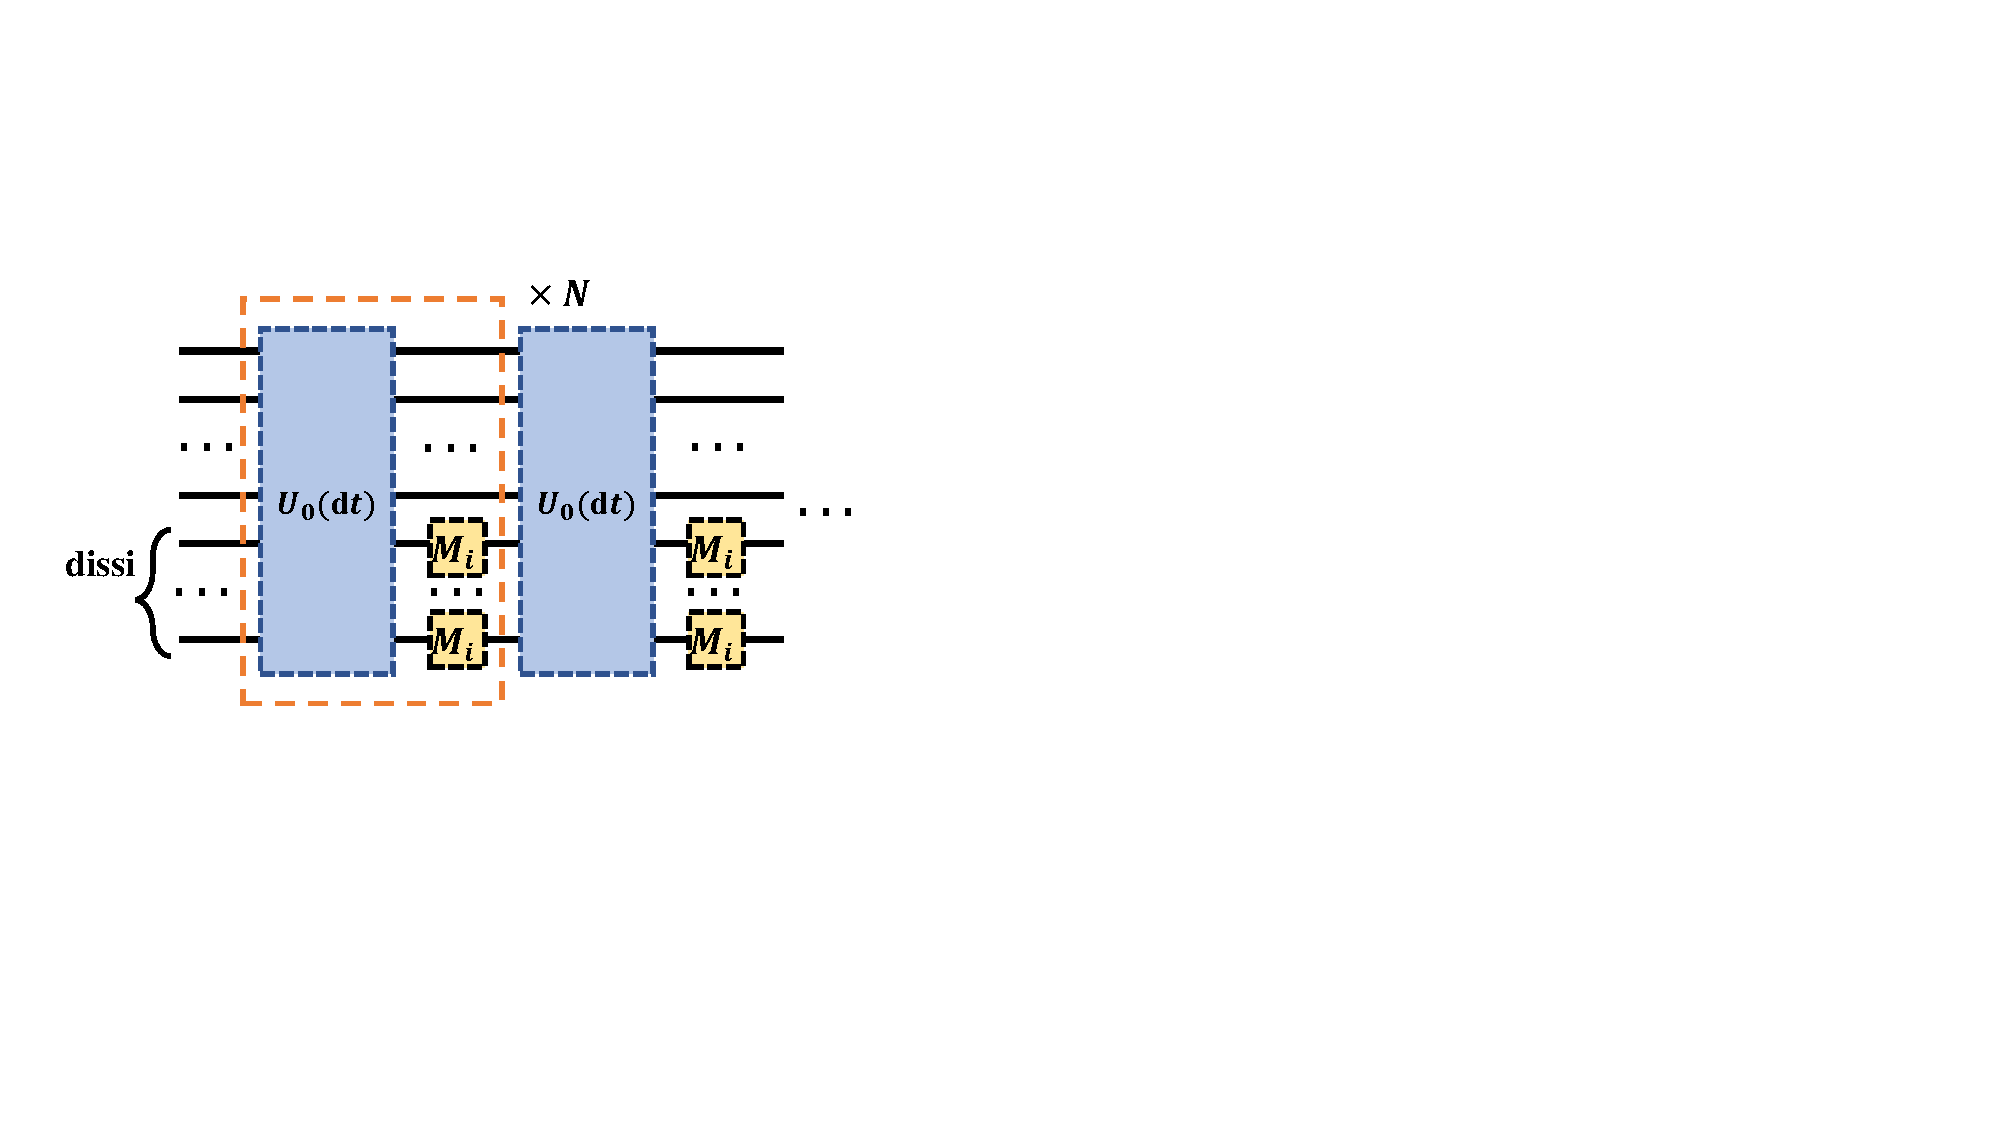
\includegraphics[width=1.\linewidth]{Picture/Circuit.pdf}
		\caption{实现增益/耗散非厄米哈密顿量的受控量子线路的示意图，每一个比特代表晶格的一个格点，厄米部分的时间演化$U_0(\mathrm{d}t)$通过量子门实现。作用耗散格点非厄米部分的时间演化通过广义测量实现，在图中标记为'dissi'。作用$N$层演化之后得到$N\mathrm{d}t$时间的演化。}
		\label{fig:01}
	\end{figure}
	We propose the scheme to realize the gain/loss non-Hermitian Hamiltonian in monitored quantum circuits. The time evolution of the gain/loss non-Hermitian Hamiltonian can be realized through circuits, as depicted in Fig.~\ref{fig:01}. The non-Hermitian Hamiltonian $\hat{H}_{\text{non}}$ consists of Hermitian part $\hat{H}_0$, such as the Hamiltonian of Qi-Wu-Zhang (QWZ) model which will be introduced below, and non-Hermitian part $\hat{H}_{\text{im}}$,
	\begin{equation}
		\hat{H}_{\text{non}} = \hat{H}_0 +\hat{H}_{\text{im}}. \label{eq:non-hermitian}
	\end{equation}
	The non-Hermitian part $\hat{H}_{\text{im}}$ is the sum of gain/loss energy on each site, which holds imaginary onsite energy, such as $\hat{H}_{\text{im}} = \sum_{i\in \text{dissi}} \mathrm{i}\tilde{\gamma} \hat{c}_i^{\dagger} \hat{c}_i$ for dissipative (gain) energy. The time evolution of non-Hermitian part can be realized through generalized measurements $M_i$, as shown in Sec.\ref{sec:method}. The time evolution of Hermitian part $U_0(\mathrm{d}t)$ can be realized through quantum gates. The effective dynamics of this monitored quantum circuit and the realization of the generalized measurements $M_i$ are shown in Sec.\ref{sec:method}.


	\subsection{single-excitation subspace}

	% 我应该从多体的背景出发来得到新的现象。不过只是承接关系改一下。

	We take chiral skin effect as an prominent example to study our scheme. We consider the Qi-Wu-Zhang (QWZ) model with Hamiltonian
	\begin{align}
		\hat{H}_{\text{QWZ}} &=  \sum_{{x}=1}^{L_{x}-1} \sum_{{y}=1}^{L_{y}}\left(\hat{c}_{{x}+1, {y}}^{\dagger} \hat{c}_{{x}, {y}} \otimes \frac{\hat{\sigma}_{z}+i \hat{\sigma}_{x}}{2}+\mathrm{H.c.}\right) \notag\\
		& +\sum_{{x}=1}^{L_{x}} \sum_{{y}=1}^{L_{y}-1}\left(\hat{c}_{{x}, {y}+1}^{\dagger} \hat{c}_{{x}, {y}} \otimes \frac{\hat{\sigma}_{z}+i \hat{\sigma}_{y}}{2}+\mathrm{H.c.}\right) \notag\\
		& +u \sum_{{x}=1}^{L_{x}} \sum_{{y}=1}^{L_{y}} \hat{c}_{{x}, {y}}^{\dagger} \hat{c}_{{x}, {y}} \otimes \hat{\sigma}_{z},
	\end{align}
	where $\hat{c}_{{x}, {y}}^{\dagger}$ ($\hat{c}_{{x}, {y}}$) is the creation (annihilation) operators at site $({x},{y})$. The system has $L_x$ ($L_y$) unit cells in x-direction (y-direction) and each unit cell has two sites, labeled as $A$ and $B$.
	When the boundary of the system are dissipative or gain, the system will have chiral skin mode. This topological phenomena can be studied by the monitored quantum circuits, as depicted in Fig.~\ref{fig:01}. 

	% We show the spectrum and chiral skin mode of non-Hermitian Hamiltonian and the effective Hamiltonain of the MQC in Fig.~\ref{fig:02}. The results of non-Hermitian Hamiltonian are shown in Fig.~\ref{fig:02} (a) and (c) and the results of the effective Hamiltonian are shown in Fig.~\ref{fig:02} (b) and (d). The complex energy spectrum in Fig.~\ref{fig:02} (a) and Fig.~\ref{fig:02} (b) is the same. The results in Fig.~\ref{fig:02} (c) and (d) show the chiral skin mode whose complex energy is labeled with a red cross in Fig.\ref{fig:02} (a) and (b). The results in Fig.~\ref{fig:02} show the correctness of our scheme.  % 太多引用Fig和

	In the following, we will show that the chiral skin modes appear when the measurement is applied on $y=1$ boundary of the system. We compare the spectrum and chiral skin mode of the QWZ model ($u=-1.5, L_x=L_y=40$) between non-Hermitian system and our measurement schemes in Fig.~\ref{fig:02}. The results of Fig.~\ref{fig:02} (a), Fig.~\ref{fig:02} (b) are calculated from non-Hermitian Hamiltonian $\hat{H}_{\text{QWZ}} + \hat{H}_{\text{im}}$ , the effective Hamiltonian $\hat{H}_{\text{eff}}^{(N)}$ of the  scheme in Eq.\ref{eq:H_scheme1} respectively. 
	%In this and the following sections, 
	The spectrum and chiral skin modes are obtained from exact diagonalization calculations. The results in Fig.~\ref{fig:02} show the correctness of our scheme.

	\begin{figure}[h]
		\centering
		\begin{overpic}[width=1.0\linewidth]{Picture/SingleExcitation_Comp.pdf}
			\put(7,97){(a)}
			% \put(7,54){(c)}
			\put(49,97){(b)}
			% \put(49,54){(d)}
		\end{overpic}
		%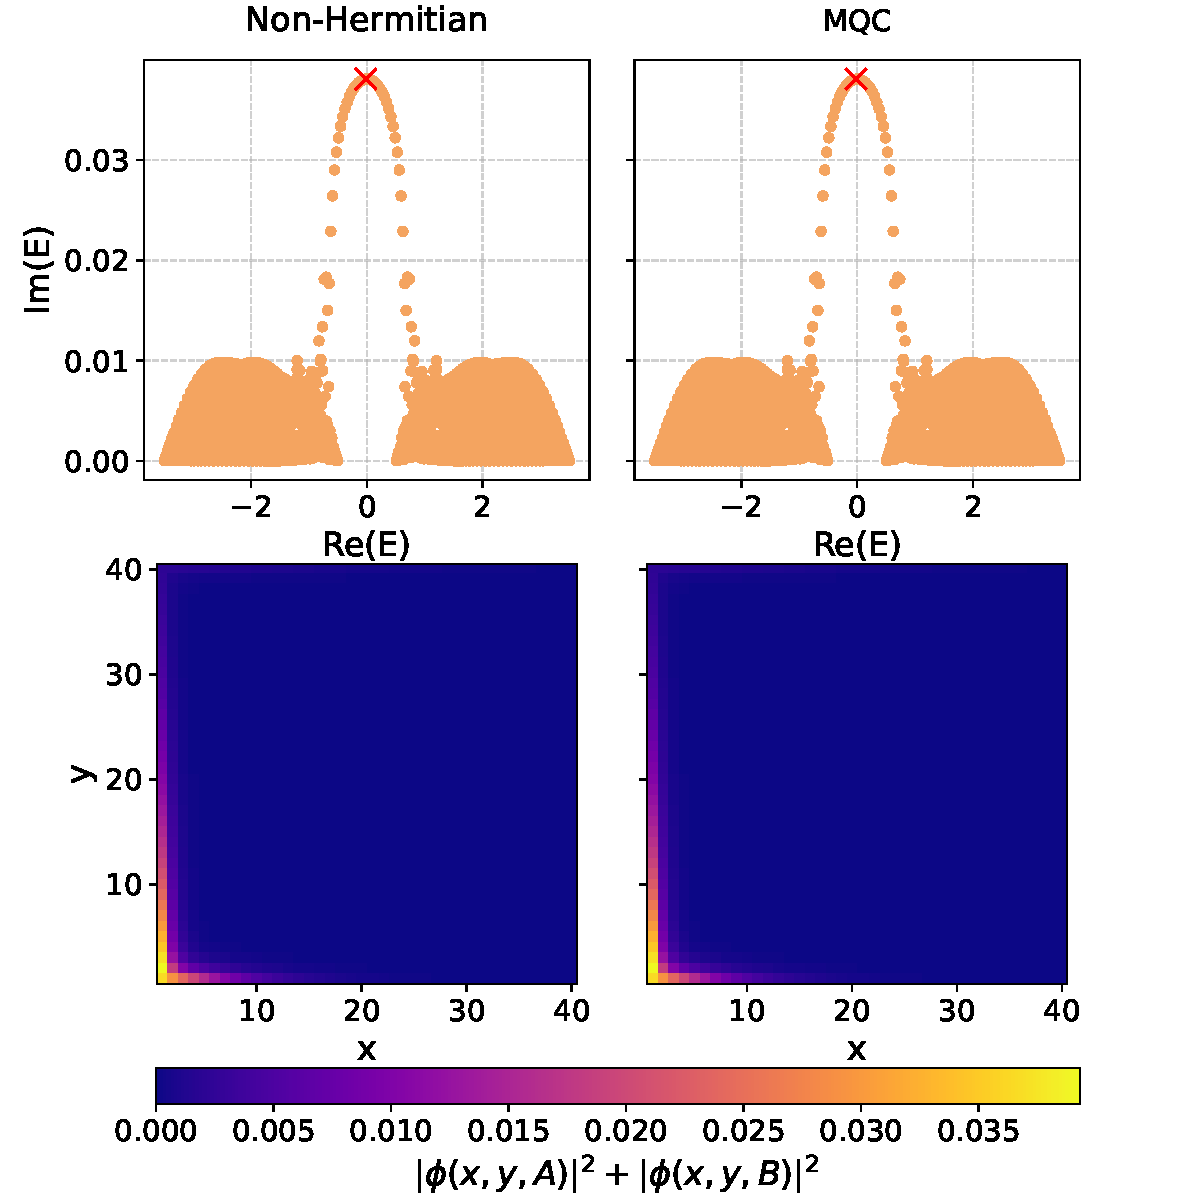
\includegraphics[width=1.\linewidth]{Picture/SingleExcitation_Comp.pdf}
		\caption{在单激发子空间中能谱和本征态对比。(a) 非厄米哈密顿量的能谱和本征态在各元胞的粒子数。 (b) MQC的有效哈密顿量$\hat{H}_{\mathrm{eff}}^{(N)}$的能谱和本征态在各元胞的粒子数。 该本征态是chiral skin mode，其能量在能谱中用红色十字标记。系统尺寸为$L_x=L_y=40$，非厄米参数为$\gamma=0.2$，在位能为$u=-1.5$。MQC的参数为$N=200$, $\mathrm{d}t$=0.001。}
		\label{fig:02}
	\end{figure} %label from y=1 and x=1?


	\subsection{Double-excitation subspace}

	\begin{figure}[h]
		\centering
		%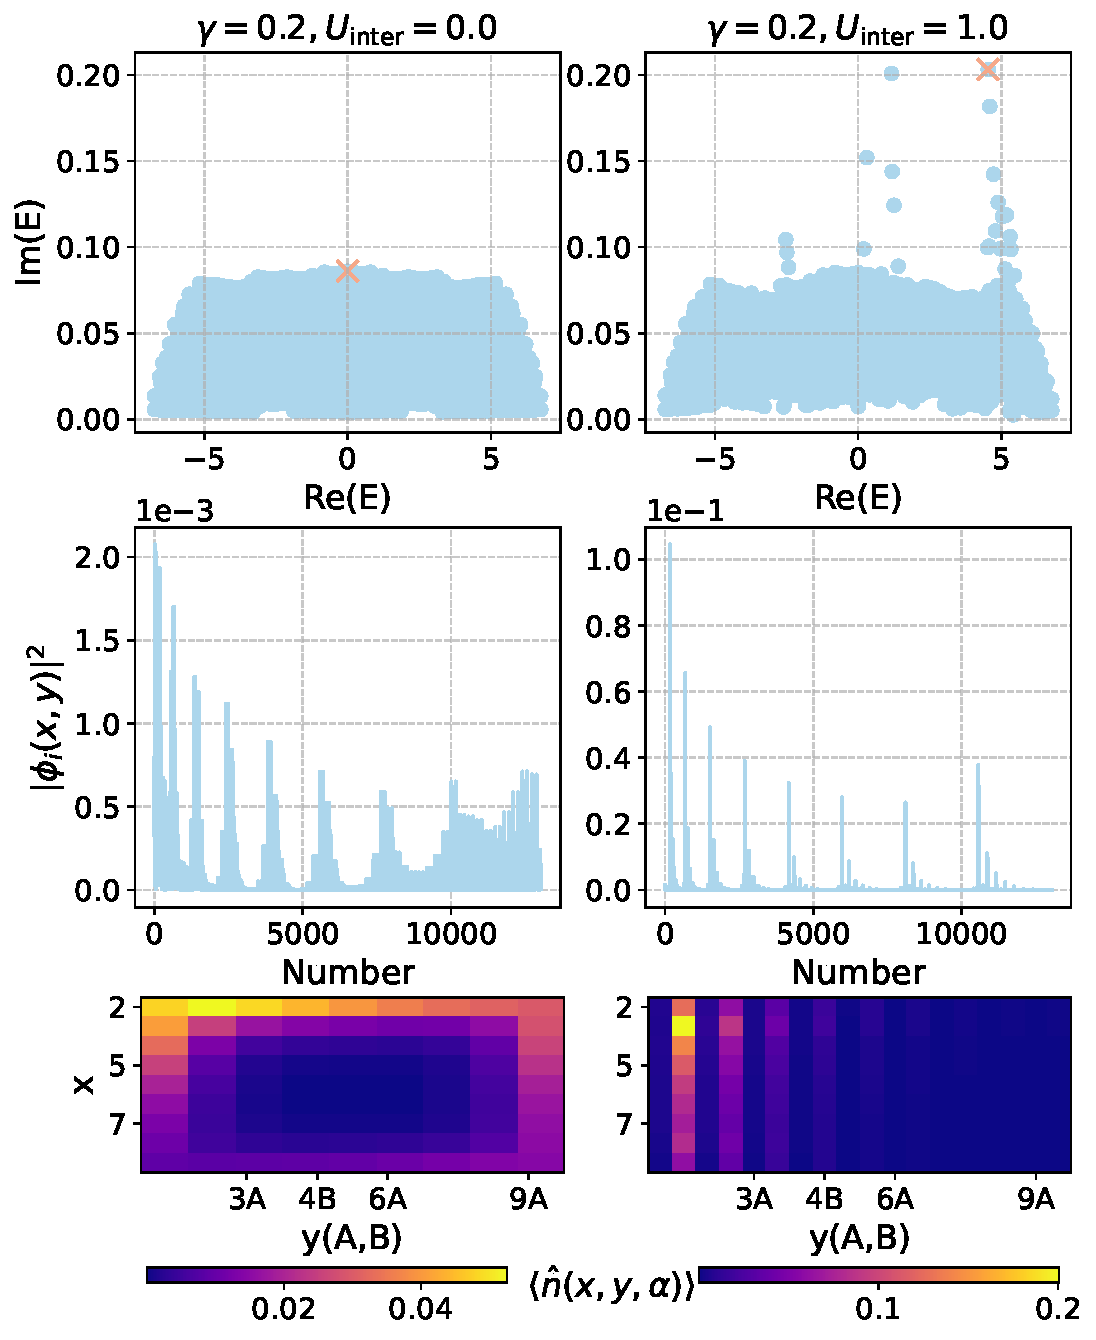
\includegraphics[width=1.\linewidth]{Picture/TwoExcitationSpectrum.pdf}
		\begin{overpic}[width=1.0\linewidth]{Picture/TwoExcitationSpectrum.pdf}
			\put(6,97){(a)}
			\put(44,97){(b)}
			% \put(7,54){(c)}
			\put(6,63){(c)}
			\put(44,63){(d)}
			\put(6,27){(e)}
			\put(44,27){(f)}
			% \put(49,54){(d)}
		\end{overpic}
		\caption{在双激发子空间中能谱和本征态对比，非厄米增益$\hat{H}_{\text{im}}$作用于$y=1$边界的元胞。(a) 在不存在相互作用和(b) 存在相互作用时的能谱。(c) 在不存在相互作用和(d) 存在相互作用时本征态的模方，其能量在(a)和(b)中用橘色十字表示。(e) (c)中本征态在各个格点的粒子数平均数，该态是多粒子的chiral skin mode。(f) (d)中本征态在各个格点的粒子数平均数，该态是NHMBL。系统尺寸为$L_x=L_y=9$，在位能为$u=-1.5$。}
		\label{fig:03}
	\end{figure}

	% \begin{figure}[h]
	% 	\centering
	% 	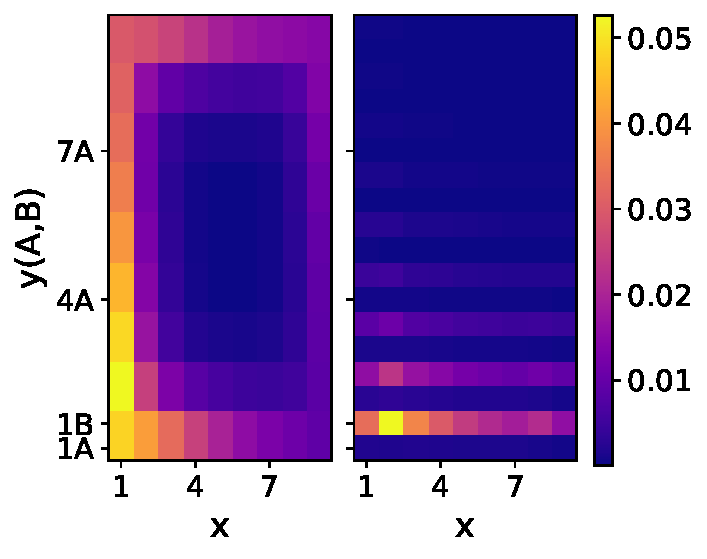
\includegraphics[width=0.6\linewidth]{Picture/TwoExcitation_Eigen.pdf}
	% 	\caption{}
	% 	\label{fig:03} % 颜色 应该归一化。
	% \end{figure}

	当研究多粒子系统时，chiral skin 效应在多体相互作用存在时是否仍然存在，以及多体相互作用与环境引入的非厄米是否共同导致特有的局域效应，仍然是尚未解决的问题。我们在双激发子空间中，对不存在相互作用和存在相互作用增益非厄米哈密顿量进行了计算，相应的能谱和本征态展示在Fig.~\ref{fig:03}中。我们这里以元胞间的相互作用为例
	\begin{widetext}
		\begin{align}
			\hat{H}_{\text{inter}} = &\sum_{{x}=1}^{L_{x}-1} \sum_{{y}=1}^{L_{y}}  U_{\text{inter}} \left(\hat{n}_{{x}, {y}, A}+\hat{n}_{{x}, {y}, B}\right) \left(\hat{n}_{{x}+1, {y}, A}+\hat{n}_{{x}+1, {y}, B}\right)\\
			& + 
			\sum_{{x}=1}^{L_{x}} \sum_{{y}=1}^{L_{y}-1}  U_{\text{inter}} \left(\hat{n}_{{x}, {y}, A}+\hat{n}_{{x}, m_y, B}\right) \left(\hat{n}_{{x}, {y}+1, A}+\hat{n}_{{x}, {y}+1, B}\right),
		\end{align}
	\end{widetext}
	where $\hat{n}_{{x},{y},\alpha}=\hat{c}_{x,y,\alpha}^{\dagger}\hat{c}_{x,y,\alpha}$ is the number operator at $\alpha$ sublattice of unit cell (${x},{y}$).
	当没有相互作用时，多粒子空间的chiral skin mode可以通过单粒子量子态进行构造，因此多个chiral skin mode构造的多粒子态仍然会呈现出chiral skin effect，如Fig.~\ref{fig:03} (c)展示了无相互作用下的手性趋肤模式。
	% 但是泡利排斥阻止所有粒子在同一个角落上积累。

	当系统存在相互作用$\hat{H}_{\text{inter}}$时，相应的能谱和最大虚本征值的本征态如Fig.~\ref{fig:03}第二列所示。Fig.~\ref{fig:03}(c) and (d) 展示了双激发子空间中最大虚本征值的本征态，其复能量在Fig.~\ref{fig:03}(a) and (b)中用橘色十字表示。Fig.~\ref{fig:03}(c)展示了两粒子的chiral skin mode，Fig.~\ref{fig:03}(d)则是由于环境导致的增益和多体相互作用导致的非厄米多体局域态。为了显示多体量子态的局域性，我们计算多体量子态在每个格点上的平均粒子数，也就是
	\begin{equation}
		\langle \hat{n}(x,y,\alpha) \rangle = \langle \phi_i \vert \hat{n}_{x,y,\alpha} \vert \phi_i \rangle,
	\end{equation}
	其中$\phi_i$表示量子态在双粒子子空间中的本征态，$\hat{n}_{x,y,\alpha}$is the number operator at $\alpha$ sublattice of unit cell (${x},{y}$)。在单粒子子空间，量子态的局域化能直接反应粒子数算符的局域化，因为此时基矢是单激发的，且总共只有一个粒子被激发。然而，在双粒子子空间中，量子态的局域化并不能直接反映粒子数算符的局域化。我们计算了最大虚本征值本征态在每个格点的平均粒子数，结果展示在Fig.~\ref{fig:03} (e) and (f)中。结果表明，在不存在相互作用时，本征态的粒子数算符的局域化与chiral skin mode类似，并且不区分子晶格。
	%之所以此时粒子数并不是两个单粒子chiral skin mode的粒子数之和是由于泡利排斥原理。
	在存在相互作用$\hat{H}_{\text{inter}}$时($U_{\text{inter}}$)，粒子数算符的局域化相较于无相互作用时相比时更加局域，且当相互作用$U_{\text{inter}}>0$时，粒子数算符更加局域化在$B$子晶格。
	% 出现这一现象的原因在于，

	对于不存在相互作用的非厄米哈密顿量，其本征能谱是关于复能谱中$\Re(E)=0$的直线对称的，这与单粒子子空间的结果以及以前的研究结果一致。这种对称性可以归因于$\hat{H}_{\text{QWZ}}$是在宇称和时间反演对称变换下反号，也就是anti-$\mathcal{PT}$对称的。另一方面非厄米哈密顿量$\hat{H}_{\text{im}}$在宇称变换下保持不变，但是在时间反演对称变换下反号$-\hat{H}_{\text{im}}$，因此，$\hat{H}_{\text{im}}$同样具有anti-$\mathcal{PT}$对称性，也就是
	\begin{equation}
		\begin{split}
			\mathcal{PT} \hat{H}_{\text{QWZ}} (\mathcal{PT})^{-1} = -\hat{H}_{\text{QWZ}} \\
			\mathcal{PT} \hat{H}_{\text{im}} (\mathcal{PT})^{-1} = -\hat{H}_{\text{im}}.
		\end{split}
	\end{equation}
	然而，无论是相互作用哈密顿量$\hat{H}_{\text{inter}}$are invariant under a combination of parity ($\mathcal{P}$) and time-reversal ($\mathcal{T}$) operations
	\begin{equation}
		\begin{split}
			\mathcal{PT} \hat{H}_{\text{inter}} (\mathcal{PT})^{-1} = \hat{H}_{\text{inter}}% \\
			% \mathcal{PT} \hat{H}_{\text{intra}} (\mathcal{PT})^{-1} = \hat{H}_{\text{intra}}.
		\end{split}
	\end{equation}
	对于存在anti-$\mathcal{PT}$ symmetry的系统，它的能谱是关于复能谱的$\Re(E)=0$直线对称的，这是因为
	\begin{equation}
		\begin{split}
			\hat{H} \vert \phi \rangle = E \vert \phi \rangle\\
			\mathcal{PT} \hat{H} (\mathcal{PT})^{-1} \vert \phi \rangle = - E \vert \phi \rangle\\
			\hat{H} (\mathcal{PT})^{-1} \vert \phi \rangle = - E^* (\mathcal{PT})^{-1} \vert \phi \rangle.
		\end{split}
	\end{equation}
	这表明，如果$\vert \phi \rangle$是能量为$E$的本征态，那么对于具有anti-$\mathcal{PT}$ symmetry的系统，它也存在能量为$-E^*$的本征态$\vert \phi \rangle$，因此，系统的能谱是关于复能谱的$\Re(E)=0$直线对称的。
	此外，在$\mathcal{PT}$变换下，相互作用强度为$U_{\text{inter}}$的$\hat{H}_{\text{inter}}$将变换为相互作用强度为$-U_{\text{inter}}$的$\hat{H}_{\text{inter}}$。
	%和$\hat{H}_{\text{intra}}$
	因此，具有相互作用强度为$U_{\text{inter}}$的多体哈密顿量的能谱和本征态与相互作用为$-U_{\text{inter}}$的多体哈密顿量的能谱和本征态之间存在对称性
	\begin{equation}
		\begin{split}
			\mathcal{PT} (\hat{H}_{\text{QWZ}}+\hat{H}_{\text{inter}}\vert_{U_{\text{inter}}}+\hat{H}_{\text{im}}) (\mathcal{PT})^{-1}\\
			= -(\hat{H}_{\text{QWZ}}+\hat{H}_{\text{inter}}\vert_{-U_{\text{inter}}}+\hat{H}_{\text{im}}).
		\end{split}
	\end{equation}
	相互作用$U_{\text{inter}}$的系统的本征值和本征态分别为可以表示为$\{E_{\text{inter}}\}$和$\{\phi_{\text{inter}}\}$，相互作用$-U_{\text{inter}}$的系统的本征值和本征态则为$\{-E^*_{\text{inter}}\}$和$\{(\mathcal{PT})\phi_{\text{inter}}\}$。
	%是否可以加一个表格说明，chiral skin 在什么时候会出现，什么子空间会出现。同时后面还要解释是关于sublattice对称的不。
	\begin{table*}[htbp]
		\centering
		\caption{The comparison of between chiral skin mode and NHMBL in many-body excited subspace. The 'yes' means the phenomena exists and 'yes' means the phenomena does not exist. }
		\begin{tabular}{l|p{2cm}p{3cm}p{3cm}p{2cm}p{2cm}}
		%   \toprule  % 顶部线
		\hline
		  phenomena & with $\hat{H}_{\text{inter}}$ & dissipative bulk & $u<-2$($u>2$) & with $\hat{H}_{\text{intra}}$ & $\gamma<0$\\
		%   \midrule  % 中部线
		\hline
		  chiral skin mode & no & no & no & yes & yes\\
		  NHMBL & yes & yes & yes & no & yes\\
		%   \bottomrule % 底部线
		\hline
		\end{tabular}
		\label{tab:example}
	\end{table*}

	\begin{figure}[h]
		\centering
		%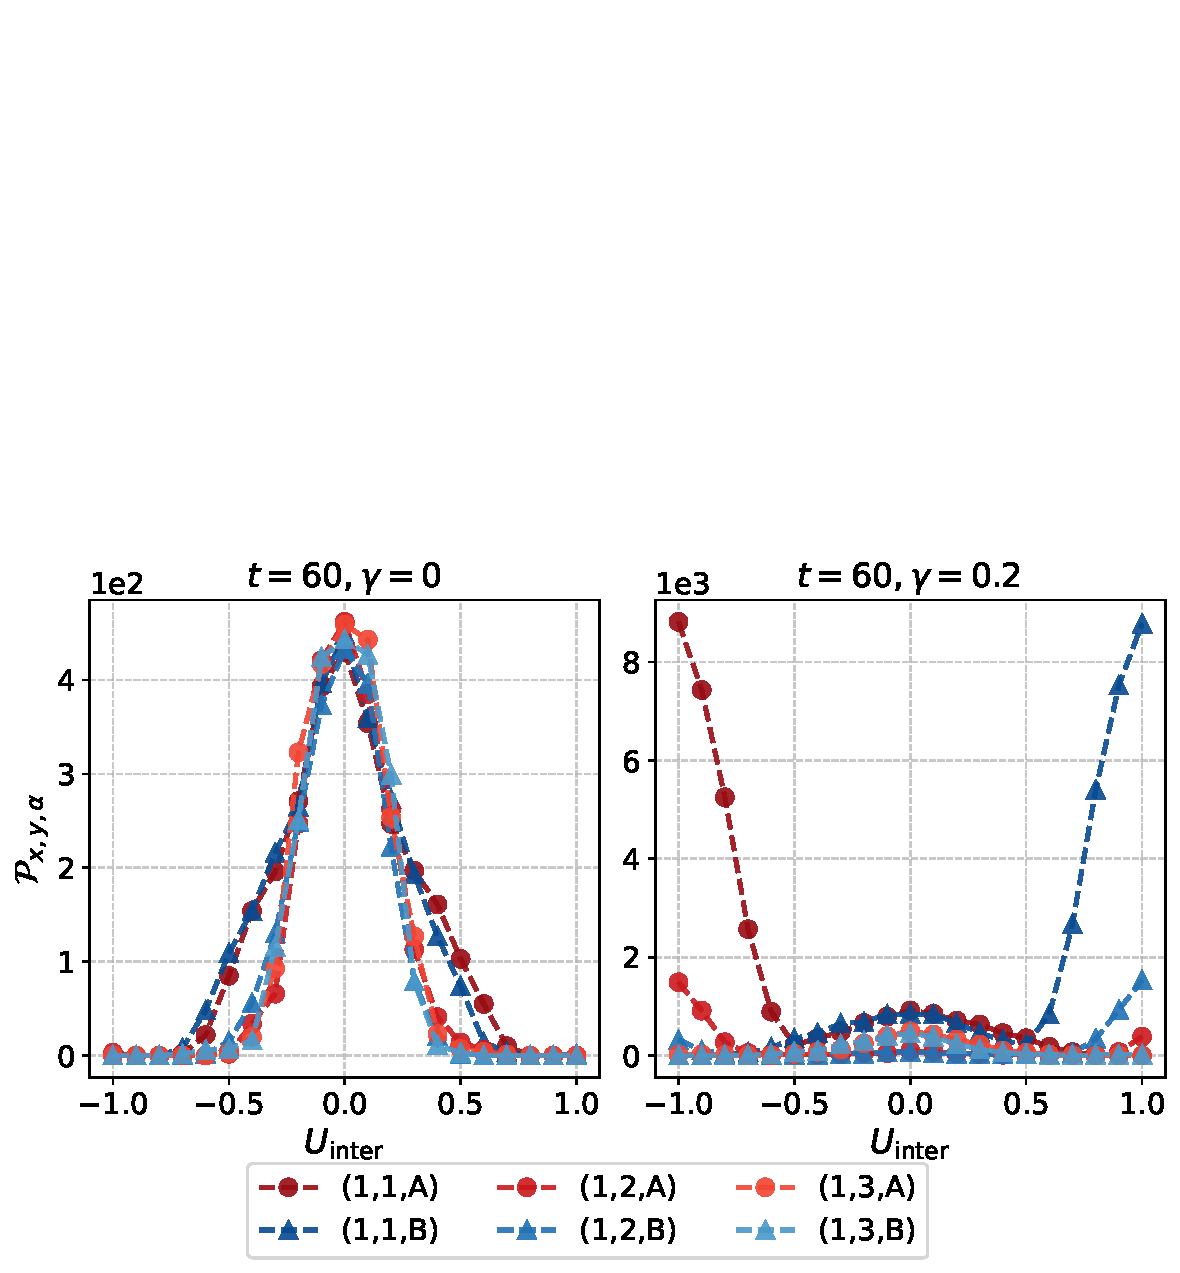
\includegraphics[width=1.\linewidth]{Picture/Popu_Interaction.pdf}
		\begin{overpic}[width=1.0\linewidth]{Picture/Popu_Interaction.pdf}
			\put(3,60){(a)}
			\put(50,60){(b)}
			% \put(49,54){(d)}
		\end{overpic}
		\caption{在时间$t=60$时，不同相互作用强度下的$\mathcal{P}_{x,y,\alpha}$。(a) 不存在非厄米增益的多体哈密顿量。(b) 存在$\gamma=0.2$的$\hat{H}_{\text{im}}$的多体非厄米哈密顿量，增益作用于$y=1$元胞。系统尺寸为$L_x=L_y=7$，在位能为$u=-1.5$。选取的随机初始量子态数目为$N_{\text{samp}}=10^4$。}
		\label{fig:04}
	\end{figure} % 可以只保留下面两个。其它放在appendix中。
	To study the non-Hermitian-driven many-body localization (NHMBL) in different interaction strength $U_{\text{inter}}$, we defined a quantity that is friendly to the monitored quantum circuits. % 我们定义了一种适合于量子电路监测的量度。
	我们首先在线路中随机激发两个格点，并计算不含和含多体相互作用$\hat{H}_{\text{inter}}$的非厄米哈密顿量的时间演化，该演化可以通过Fig.~\ref{fig:01}所示的量子线路实现。然后，在时间$t=60$时，探测末态$\psi_t$每个格点的平均粒子数$\langle \psi_{t} \vert \hat{n}_{x,y,\alpha} \vert \psi_t \rangle$，其中$\alpha=A(B)$表示$A(B)$子格点。我们进行了$N_{\text{samp}}=10^{4}$次实验，并在每次实验统计每个格点$\langle \psi_{t} \vert \hat{n}_{x,y,\alpha} \vert \psi_t \rangle$大于$1/(2L_x)$的事件数
	\begin{equation}
		\mathcal{P}_{{x}, {y}, {\alpha}} = \sum_{N_{\text{samp}}} \mathbb{I}(\langle \psi_{t} \vert \hat{n}_{x,y,\alpha} \vert \psi_t \rangle > \frac{1}{2L_x}).
	\end{equation}
	where $\mathbb{I}(X)$ is the indicator function, which is 1 (0) when X is true (false).% 其中，$\mathbb{I}(X)$是指示函数，当$X$为真时取值为1，否则取值为0。
	结果表明，在多体厄米哈密顿量下，从任意一个双激发量子态出发（局域态），在时间$t=60$时，统计局域在格点$(x,y,\alpha)$的事件数$\mathcal{P}_{x,y,\alpha}$随相互作用强度$\vert U_{\text{inter}} \vert$的增加而减小，这表明随着相互作用强度的增加，量子态更趋向于演化向非局域的量子态。在存在非厄米哈密顿量时，部分格点的事件数$\mathcal{P}_{x,y,\alpha}$随着多体相互作用增强而减少，而其它格点的事件数$\mathcal{P}_{x,y,\alpha}$则表现出先减少后增加的趋势，如Fig.~\ref{fig:04}所示。我们在附录中给出了所有格点的$\mathcal{P}_{x,y,\alpha}$，得出的结论与这里一致。这是由于NHMBL，导致从任意格点出发的粒子最后都会演化到局域化的量子态，从而被探测到。在不同相互作用强度下，末态更多格点的$\mathcal{P}_{x,y,\alpha}$在Appendix.~\ref{sec:AllP}中进行详细阐述。


	% !!!这里无论如何要点出我们是从演化角度考虑的。
	接下来，我们说明，Fig.~\ref{fig:03}中的NHMBL是由增益和相互作用共同作用的结果。该机理可以通过非厄米哈密顿量的时间演化来理解。% 这需要说明与chiral skin不同，还是说明不仅是由非厄米共同导致的。
	在Fig.~\ref{fig:05}中，我们给出了不同相互作用下，仅考虑三个元胞且仅有两个粒子时的部分能级，其中蓝色波浪线表示非厄米pumping，该泵浦仅作用于前两个元胞，黑色箭头表示可能发生的跃迁，所有可能的跃迁振幅大小为$1/2$。我们在这里用$\ket{\uparrow}$表示在元胞的$A$子格点有一个粒子；用$\ket{\downarrow}$表示在元胞的$B$子格点有一个粒子。如果在Fig.~\ref{fig:05}中的某个蓝色元胞同时存在$\ket{\uparrow}$和$\ket{\downarrow}$，则表示该元胞的$A$格点和$B$格点各有一个粒子。

	对于非厄米哈密顿量，当两个粒子都位于$A$子格点或者$B$子格点时，这些态的能量是相同的(Fig.~\ref{fig:05}(a))。此时，非厄米pumping会将粒子pump到子空间
	\begin{equation}
		\mathscr{H}_{\text{pump}}=\left\{ \ket{\uparrow\uparrow0}, \ket{\downarrow\downarrow0},\ket{\uparrow\downarrow0},\ket{\downarrow\uparrow0},\ket{\underline{\uparrow\downarrow}00},\ket{0\underline{\uparrow\downarrow}0}\right\}.
	\end{equation}
	根据非厄米项的时间演化$e^{-\mathrm{i}\hat{H}_{\text{im}} \mathrm{d}t}$，由于此时粒子所在的两个元胞均存在增益，因此，相较于其它量子态，这些量子态受到的增益更强。同时，pump到空间$\mathscr{H}_{\text{pump}}$中每个量子态的强度与该态上的粒子数成正比。在非厄米哈密顿量的情况下，$\mathscr{H}_{\text{pump}}$中的量子态与不是这个空间中的量子态之间不存在能量差，因此，pump到该子空间的粒子有很大一部分会通过跃迁离开空间$\mathscr{H}_{\text{pump}}$。这导致了chiral skin effect，在经历非厄米哈密顿量的时间演化后，量子态会演化到chiral skin mode。

	当存在多体相互作用时，非厄米pumping同样会将粒子pump到空间$\mathscr{H}_{\text{pump}}$中的量子态，然而，在存在多体相互作用$\hat{H}_{\text{inter}}$时，该空间中的量子态与能跃迁到的其它能级之间至少存在$U$的能级差，因此被pump到该空间的粒子跃迁到该空间之外的几率更低，从而导致局域化现象的出现。与存在多体相互作用$\hat{H}_{\text{inter}}$时不同，不存在$\hat{H}_{\text{inter}}$时出现的是一种非厄米拓扑效应，这种效应仅在QWZ模型是拓扑绝缘体时才会存在，即当$-2<u<0$和$0<u<2$。然而，由增益/耗散和多体相互作用共同作用引起的多体局域化现象并不依赖于拓扑绝缘体的存在，相关讨论已在Appendix.~\ref{sec:NHMBL}中进行详细阐述。因此，这两种局域化现象的机制是完全不同的。对于含元胞内多体相互作用的非厄米哈密顿量
	\begin{equation}
		\hat{H}_{\text{intra}} = \sum_{{x}=1}^{L_{x}-1} \sum_{{y}=1}^{L_{y}}  U_{\text{intra}} \hat{n}_{{x}, {y}, A} \hat{n}_{{x}, {y}, B},
	\end{equation}
	where $U_{\text{intra}}$ is the interaction strength. 
	此时多粒子空间的局域态与不存在多体相互作用时类似，$\mathscr{H}_{\text{pump}}$中的部分能级与能跃迁到的能级之间不存在能级差，因此在这种多体相互作用的非厄米哈密顿量下，同样只可能观察到chiral skin effect，相关讨论已在Appendix.~\ref{sec:NHMBL_intra}中详细阐述。
	

	当相互作用强度$U_{\text{inter}}>0$时，多粒子经过时间演化后，更容易演化到能级$\ket{\downarrow\downarrow0}$而非$\ket{\uparrow\uparrow0}$，这是因为能跃迁到能级$\ket{\downarrow\downarrow0}$的能级更多且能级差更小。因为非厄米pump的强度与粒子在该态上的概率成正比，因此粒子更倾向于演化到能级$\ket{\downarrow\downarrow0}$，也就是$B$子晶格(Fig.~\ref{fig:03} (f))。在二维晶格中，我们在$y=1$的元胞施加增益，经过类似的分析可以得出，当存在多体相互作用$\hat{H}_{\text{inter}}$时，量子态会出现局域化，并且粒子更倾向于局域在$y=1$元胞的$B$子格点上。进一步得，从任意双激发量子态出发，经过时间$t=60$的演化后的末态更容易在$(1,1)$元胞的$B$格点上表现出局域化信号，通过粒子数算符测量，约$88\%$的实验中可以在该格点测量到粒子数的平均值大于$1/(2L_x)$（Fig.~\ref{fig:04}）。
	% 正比于在该量子态上的概率
	% 多体相互作用会使量子态更加不局域吗？这一段我觉得还有很多可以优化的空间。
	\begin{figure}[h]
		\centering
		% 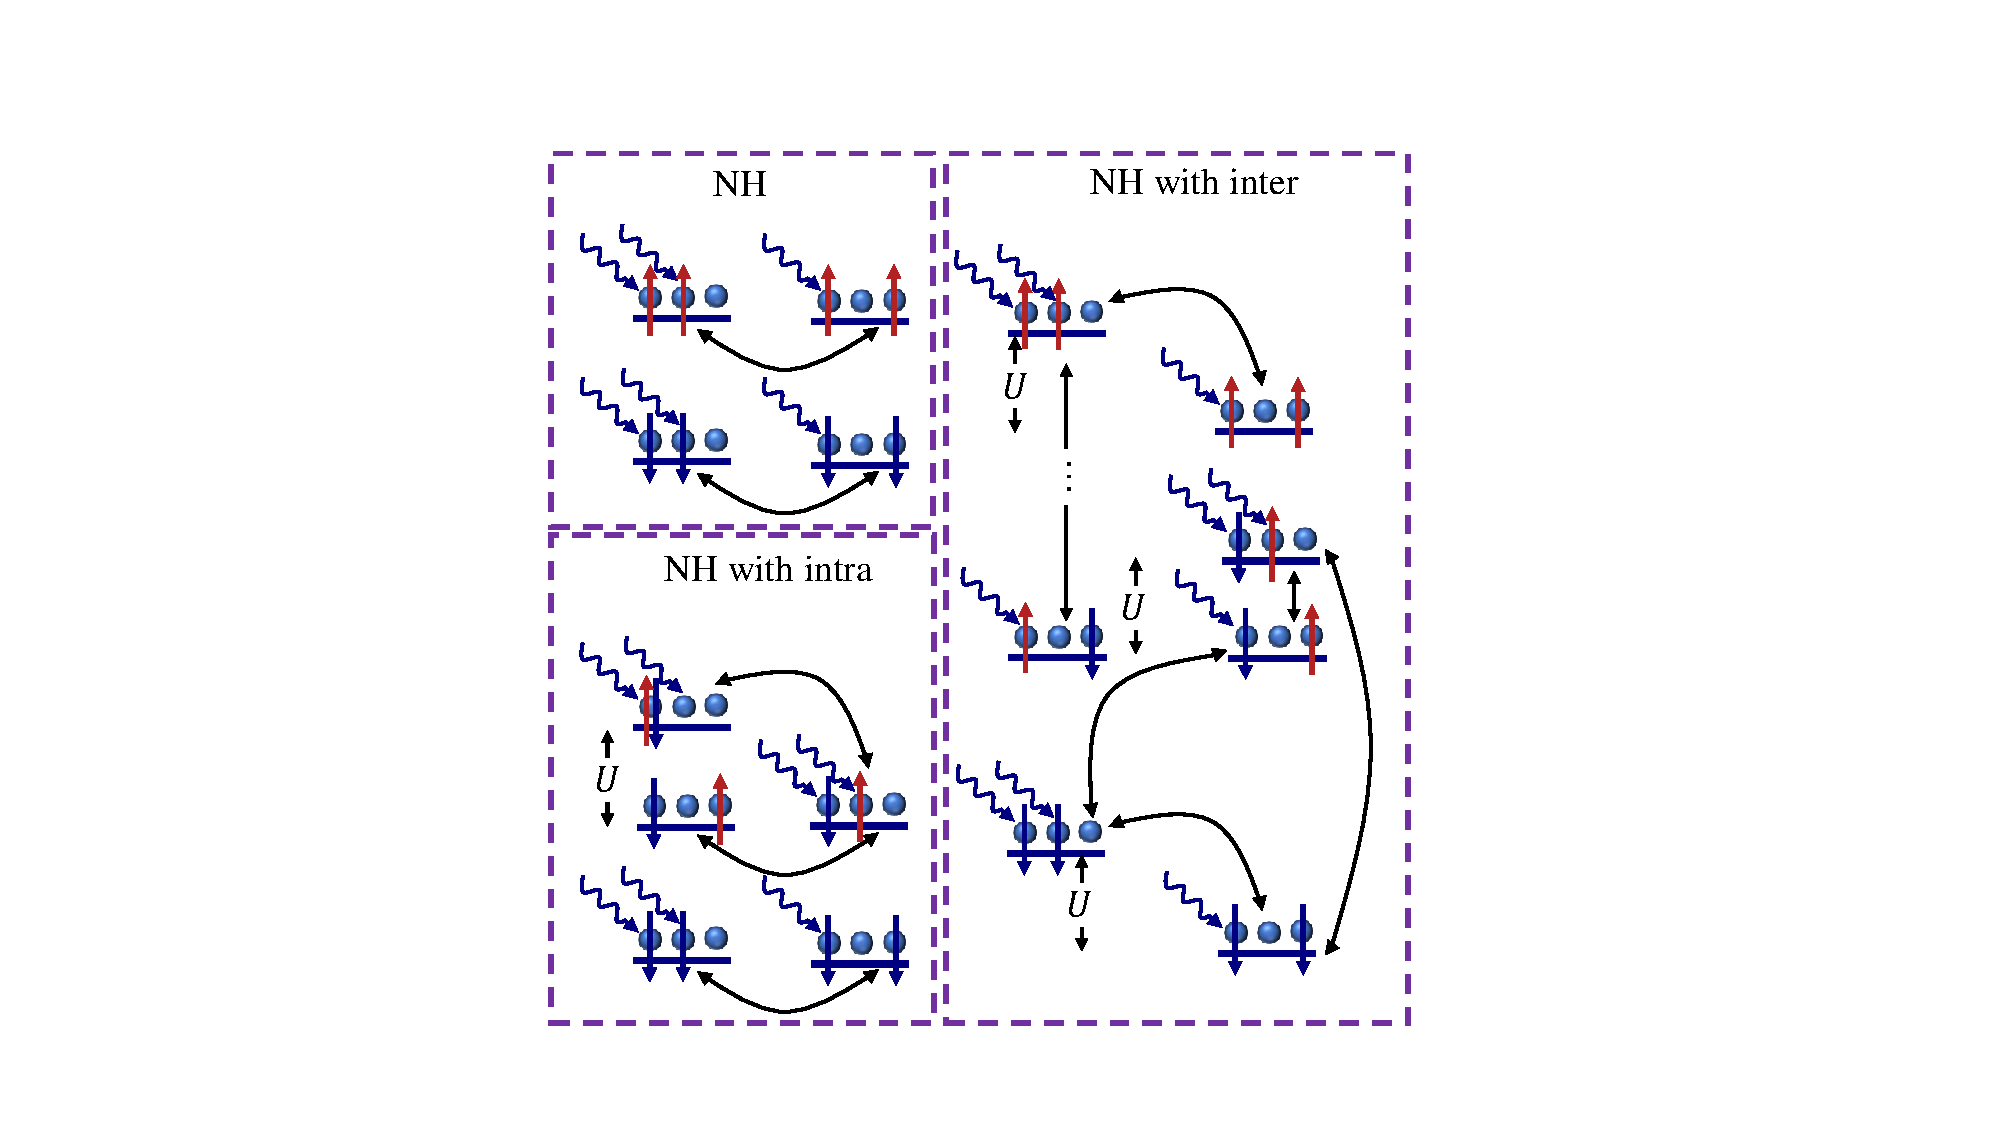
\includegraphics[width=1.0\linewidth]{Picture/Mechanism_inter.pdf}
		\begin{overpic}[width=1.0\linewidth]{Picture/Mechanism_inter.pdf}
			\put(2,94){(a)}
			\put(48,94){(b)}
			% \put(7,54){(c)}
			\put(2,52){(c)}
			% \put(49,54){(d)}
		\end{overpic}
		\caption{(a) 在不存在相互作用、(b)存在相互作用$\hat{H}_{\text{inter}}$和(c) 存在相互作用$\hat{H}_{\text{intra}}$的非厄米哈密顿量的双激发子空间部分量子态示意图。每个蓝色圆球表示一个元胞，元胞上的蓝色向下箭头表示在该元胞的$B$子格点有一个粒子，红色向上箭头表示在该元胞的$A$子格点有一个粒子，黑色箭头表示允许的量子跃迁。蓝色波浪箭头表示非厄米pumping，它表示在经历时间演化之后粒子会被pump到这些量子态，蓝色波浪线箭头的数目代表pump的强度。$U$表示由于相互作用导致出现的能级差。}
		\label{fig:05}
	\end{figure} % 需要说明一下非厄米是什么情况吗？

	\subsection{Three-excitation Subspace}

	上述分析和计算可以拓展到更多粒子激发的子空间。我们考虑了一个大小为$L_x=L_y=5$的二维晶格。为了计算方便，我们考虑三激发的子空间。在Fig.~\ref{fig:06}中，我们展示了非厄米哈密顿量和非厄米多体哈密顿量的能谱、最大虚本征值的本征态以及该态的每个格点上的粒子数算符的平均值。结果显示，非厄米哈密顿量的能谱由于anti-$\mathcal{PT}$对称性，表现出关于能谱虚轴的对称性，然而，当引入多体相互作用时，该对称性不再成立。
	与之前的分析一致，随着多体相互作用的引入，本征态以及粒子数算符的平均值都表现出局域化现象。需要注意的是，由于三激发空间的计算仅限于$L_x=L_y=5$，Fig.~\ref{fig:06}(c)和(e)中非厄米哈密顿量中的本征态并非三粒子的chiral skin mode。因此，即便在更高粒子激发的子空间中，非厄米多体哈密顿量仍然表现出NHMBL。
	

	\begin{figure}[h]
		\centering
		%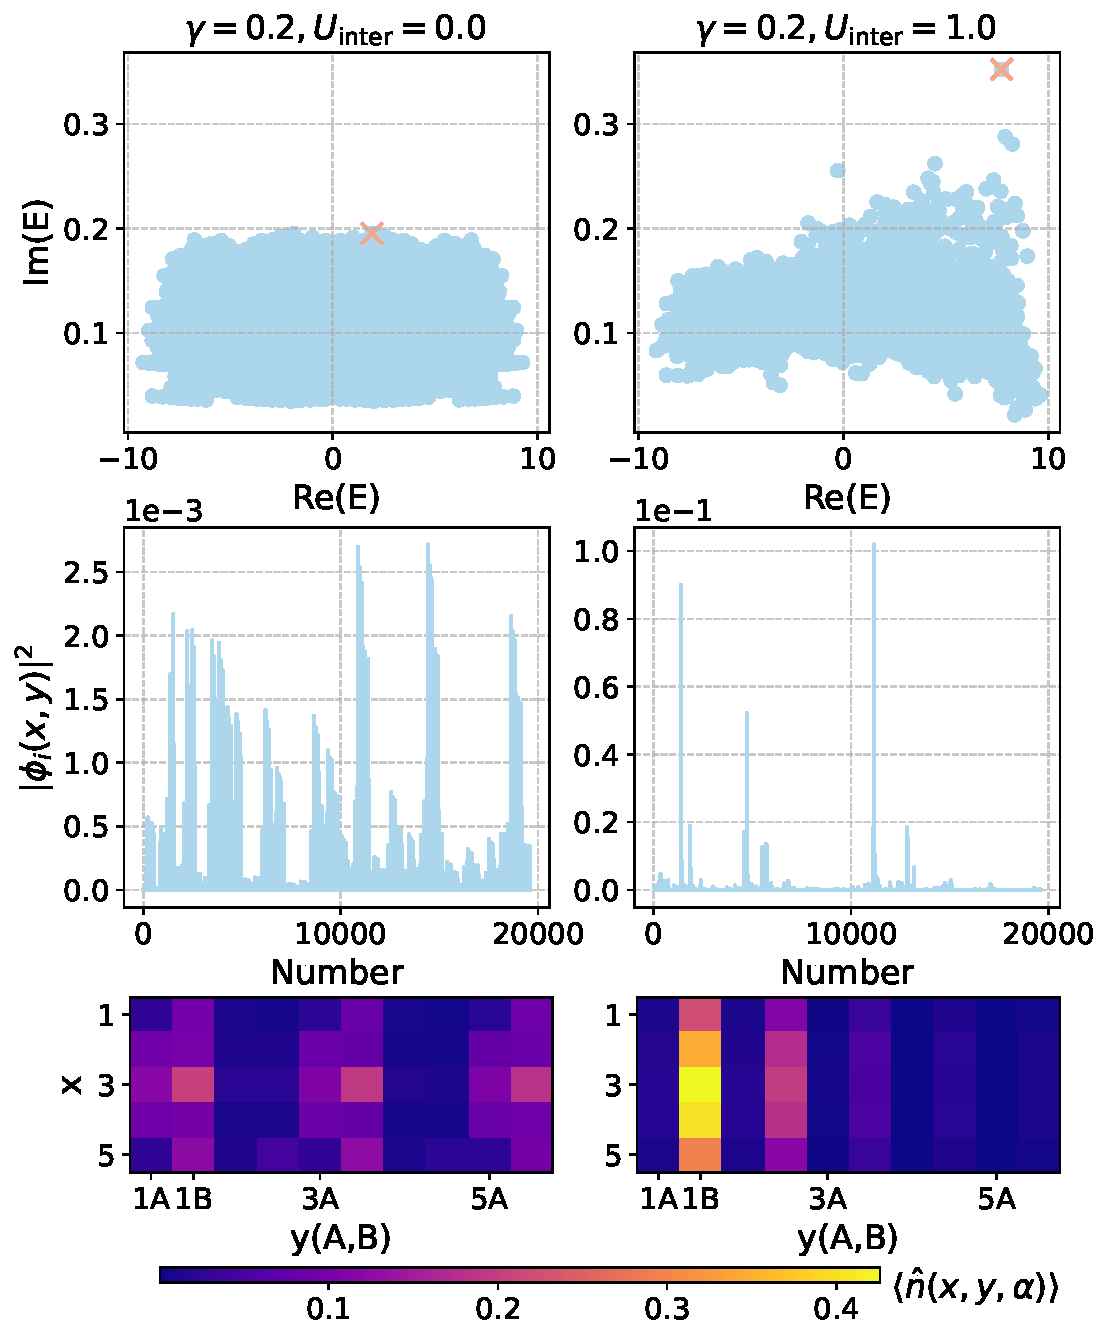
\includegraphics[width=1.\linewidth]{Picture/ThreeExcitationSpectrum.pdf}
		\begin{overpic}[width=1.0\linewidth]{Picture/ThreeExcitationSpectrum.pdf}
			\put(4,97){(a)}
			\put(42,97){(b)}
			% \put(7,54){(c)}
			\put(4,62){(c)}
			\put(42,62){(d)}
			\put(4,26){(e)}
			\put(42,26){(f)}
			% \put(49,54){(d)}
		\end{overpic}
		\caption{三激发子空间中能谱和本征态对比。(a) 在不存在相互作用和(b) 存在相互作用时的能谱。(c) 在不存在相互作用和(d) 存在相互作用时本征态的模方，其能量在(a)和(b)中用橘色十字表示。(e) (c)中本征态在各个格点的粒子数平均数，该态是多粒子的chiral skin mode。(f) (d)中本征态在各个格点的粒子数平均数，该态是NHMBL。系统尺寸为$L_x=L_y=9$，在位能为$u=-1.5$。}
		\label{fig:06}
	\end{figure}



	\subsection{Simulating the MQC in Qiskit}
	\begin{figure}[h]
		\centering
		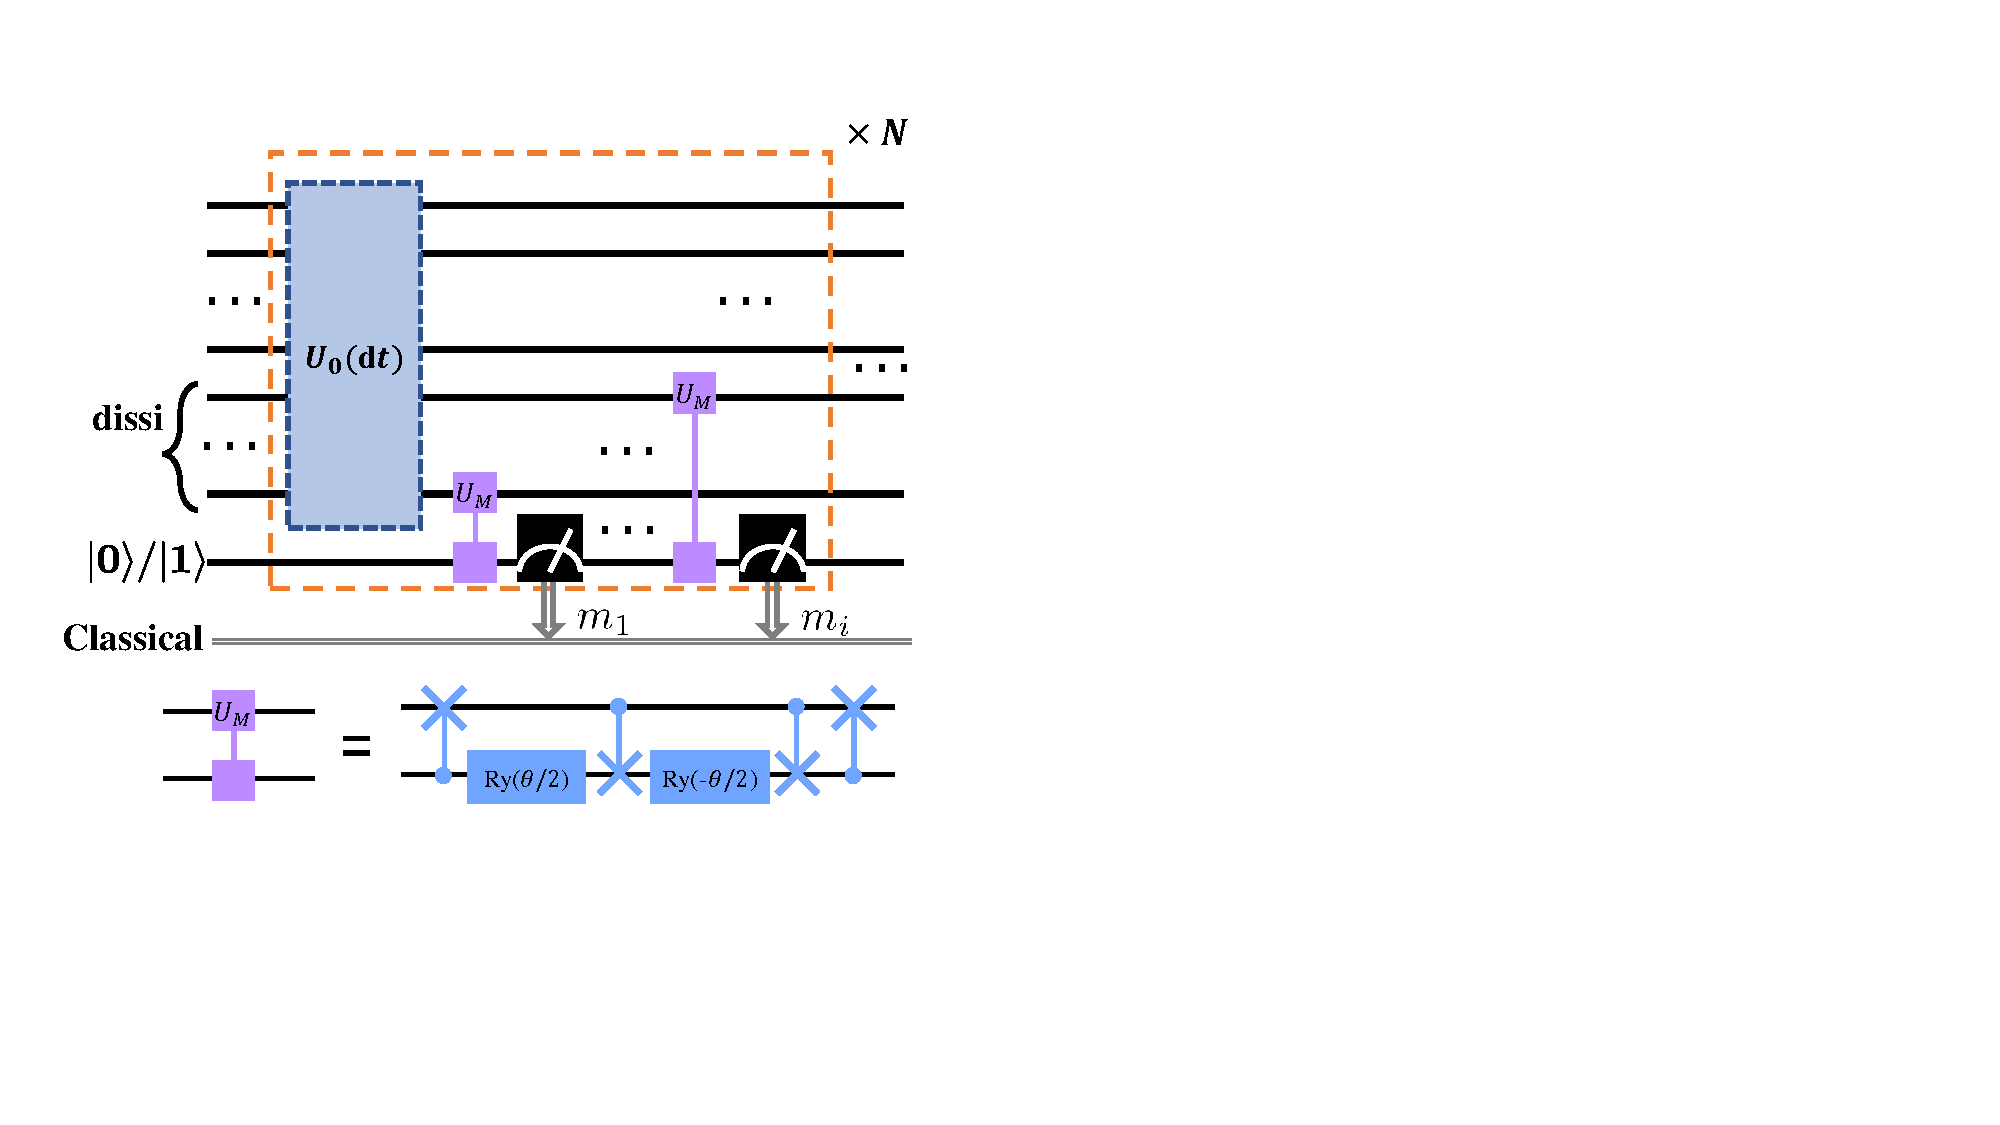
\includegraphics[width=1.\linewidth]{Picture/Circuit_Experiment.pdf}
		\caption{在Qiskit中实现增益/耗散非厄米多体哈密顿量的受控量子线路的示意图，每一个比特代表晶格的一个格点，$\ket{0}/\ket{1}$表示辅助量子比特，用来实现作用在耗散格点(标记为'dissi')的非厄米演化。厄米部分的时间演化$U_0(\mathrm{d}t)$通过量子门实现。作用$N$层演化之后得到$N\mathrm{d}t$时间的演化。作用在耗散格点和辅助比特的量子门可以通过CNOT门和单比特门实现。}
		\label{fig:07}
	\end{figure}
	% 应该可以通过一个辅助比特实现，采用Qiskit的线路。然后给出参数。
	The monitored quantum circuit for simulating non-Hermitian Hamiltonian we adapted in Qiskit is as Fig.~\ref{fig:07}. The time evolution of Hermitian part, including $\hat{H}_{\text{QWZ}}$ and many-body interaction term $\hat{H}_{\text{inter}}$, is realized through quantum gates. The time evolution of non-Hermitian part is realized through the measurements on one ancilla qubit. 
	In order to simulate the dynamics in quantum circuits, we first apply the Jordan-Wigner to the Hamiltonian. Qubit state $\ket{1}$ represents the occupation of the site and qubit state $\ket{0}$ represents the unoccupation of the site. 由于费米子对易关系的要求，我们引入一个链算符
	\begin{equation}
		P_i = \otimes_{j=1}^i\sigma^z_j.
	\end{equation}
	采用$\sigma^-=(\sigma^x-\mathrm{i}\sigma^y)/2$和$\sigma^+=(\sigma^x+\mathrm{i}\sigma^y)/2$表示费米子算符为：
	\begin{equation}
		\begin{split}
			c_i = P_i \otimes \sigma^{-}\otimes (\otimes_{j=i+1}\sigma^0_j)\\
			c_i^{\dagger} = P_i \otimes \sigma^{+}\otimes (\otimes_{j=i+1}\sigma^0_j),
		\end{split}
	\end{equation}
	where $\sigma^{x,y,z}$ represent the Pauli matrices and $\sigma^0$ represents $2\times 2$ identity matrix. 为了通过基础的量子门实现厄米哈密顿量的演化，我们对$\hat{H}_{\text{QWZ}}$和$\hat{H}_{\text{inter}}$中的每一项进行Trotter分解来实现每一项的时间演化。
	Under the above mapping, each term of hopping term can be realized though multi-qubit gates, and each term of interaction Hamiltonian $\hat{H}_{\text{inter}}$ can be realized though two-qubit gates. All the measurements can be realized through only one ancilla. To realize the gain (loss) non-Hermitian Hamiltonian, we initialize the anciila qubit to qubit state $\ket{1}$ ($\ket{0}$). And we apply the two-qubit unitary gates $U_M$ to the dissipative sites and the ancilla qubit, as shown in Fig.~\ref{fig:07}. After applying the unitary gates, we measure the ancilla qubit and store the measurement outcomes to classical register. And we repeat the quantum circuits and realize non-Hermitian dynamics of time $N\mathrm{d}t$.
	
	The unitary gates $U_M$ can be realized through CNOT gates and $R_y(\theta) = e^{-i\sigma_y\theta}$ ($\theta = \arccos(e^{-\gamma \mathrm{d}t})$), as shown in Fig.~\ref{fig:07}. 我们选择所有经典寄存器结果都是$\ket{1}$($\ket{0}$)的量子轨迹，可以实现增益(耗散)非厄米哈密顿量的演化。

	The comparisons between the results of the MQC and exact time-evolution are given in Fig.~\ref{fig:08}. 我们考虑一个$L_x=2,L_y=4$的二维晶格，耗散作用于$y=1$的边界上，相互作用部分为$U=1.0$的$\hat{H}_{\text{inter}}$，量子态初始的两个粒子分别位于元胞$(1,1)$的$A$格点和位于元胞$(1,2)$的$A$格点。在随后的时间对各个格点测量$\langle \hat{n}_{x,y,\alpha}\rangle$，相应的结果如图Fig.~\ref{fig:08}。它们分别是通过我们的方案的MQC和精确的方法对增益非厄米多体哈密顿量的模拟结果。它们之间的吻合表明我们的方案的MQC确实能够仅通过一个辅助比特对增益非厄米多体哈密顿量进行模拟。更多粒子的在MQC中的演化在Appendix.~\ref{sec:4Body_Evolve}中进行了详细阐述。
	\begin{figure}[h]
		\centering
		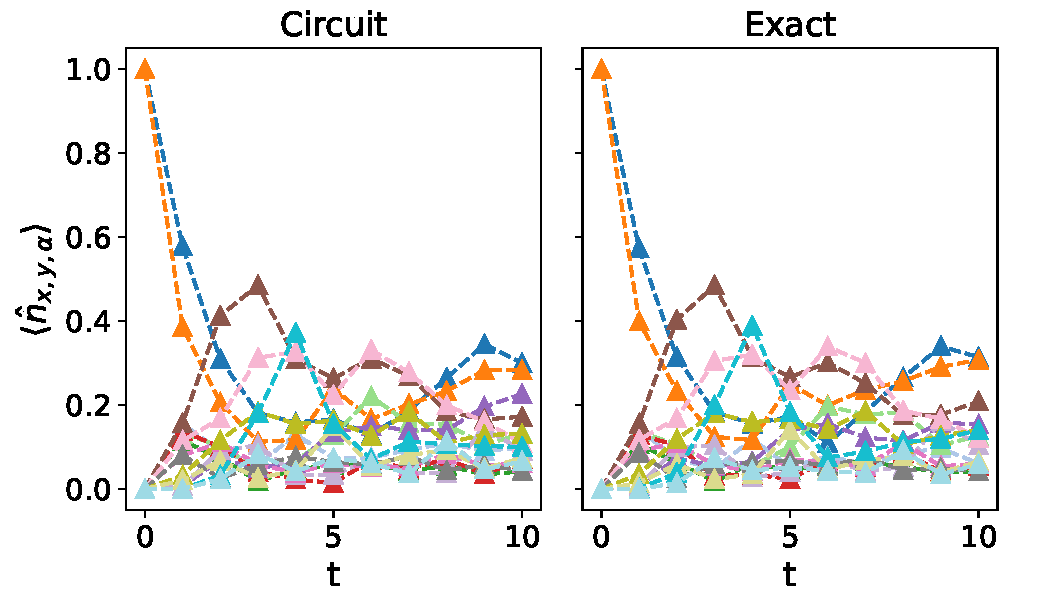
\includegraphics[width=1.\linewidth]{Picture/CircuitEvolve_ManyBody.pdf}
		\caption{从初始在元胞$(1,1)$和$(1,2)$的$A$子格点各有一个粒子开始演化，在不同时间$t$不同格点的平均粒子数。分别是通过Fig.~\ref{fig:07}的量子线路和精确计算得到的。系统尺寸为$L_x=2,L_y=4$，相互作用强度为$U_{\text{inter}}=1.0$，非厄米参数为$\gamma=0.2$。受控量子线路参数为$\mathrm{d}t=0.2$,$N=50$}
		\label{fig:08}
	\end{figure}

	\subsection{Loss Hamiltonian.}
	% 对于厄米和非厄米同样可以通过这个方式分析。对应的对称性是将x方向翻转，然后作用共轭，此时相当于chiral skin mode从一个角落到另一个角落。是对的，反时间的演化，反正这两种在MQC都很好实现。
	为了更好的理解NHMBL的物理机理，我们在前述分析中主要考虑了系统中的增益项。然而，值得注意的是，即使在仅存在耗散项的情形下，NHMBL依然存在。根据上述对机制的理解，耗散项的时间演化可被解释为将粒子从空间$\mathscr{H}_{\text{pump}}$中pump到该空间之外。该过程表面上似乎表明耗散作用不会诱导NHMBL，因为粒子最终跃迁到$\mathscr{H}_{\text{pump}}$空间之外。
	
	但是时间演化对应将量子态演化到虚本征值最大的本征态上，在考虑耗散非厄米哈密顿量时，这个本征态确实对应bulk state。但是我们还可以考虑时间反演的时间演化$e^{\mathrm{i}(\hat{H}+\hat{H}_{\text{im}})t}$，此时非厄米项对应的效果就是将粒子pump进空间$\mathscr{H}_{\text{pump}}$，在进行一段时间的时间反演演化之后，量子态会演化为局域态。我们对该非厄米哈密顿量的能谱，本征态和粒子数算符的平均值进行了数值计算，相应的结果如Fig.~\ref{fig:13}。可以发现虚本征值最小的量子态对应局域态，它对应长时间演化的稳态。
	
	此外，我们还发现，耗散系统与增益系统对应的非厄米哈密顿量之间存在对称性关系。具体而言，考虑一个沿 $y$ 方向的反射变换 $\mathcal{M}_x$。该变换将位于$x=1$的元胞映射到$x=L_x$，同时保持$y$坐标不变。在考虑多体相互作用的QWZ模型中，存在如下对称性变换关系：
	\begin{equation}
		\begin{split}
			(\mathcal{M}_x \mathcal{K})(\hat{H}_{\text{QWZ}} + \hat{H}_{\text{inter}} + \hat{H}_{im}^-) (\mathcal{M}_x \mathcal{K})^{-1} \\
			= (\hat{H}_{\text{QWZ}} + \hat{H}_{\text{inter}} + \hat{H}_{im}^+)
		\end{split}
	\end{equation}
	其中$\mathcal{K}$ denotes complex conjugate. 该对称性揭示了Fig.~\ref{fig:03}和Fig.~\ref{fig:13}之间的映射关系。Fig.~\ref{fig:03}中局域在left top的局域态，在Fig.~\ref{fig:13}局域在left bottom. 最后值得注意的是，在MQC中，时间演化和时间反演的过程均可通过通用量子门操作实现。为模拟耗散项（增益项）的非厄米的演化，我们可将ancilla制备为量子态$\ket{0}$（$\ket{1}$），并后选择测量结果为$\ket{0}$（$\ket{1}$）的量子轨迹。借助这一方案，我们也能够在MQC中实现对耗散系统中NHMBL现象的观测与验证。
	% 可以和其它结合实现虚数演化求解多体问题的本征态等中。
	\begin{figure}[h]
		\centering
		\begin{overpic}[width=1.0\linewidth]{Picture/SI/SI_TwoExcitationSpectrum_loss.pdf}
			\put(4,97){(a)}
			\put(44,97){(b)}
			% \put(7,54){(c)}
			\put(4,62){(c)}
			\put(44,62){(d)}
			\put(4,26){(e)}
			\put(44,26){(f)}
		\end{overpic}
		%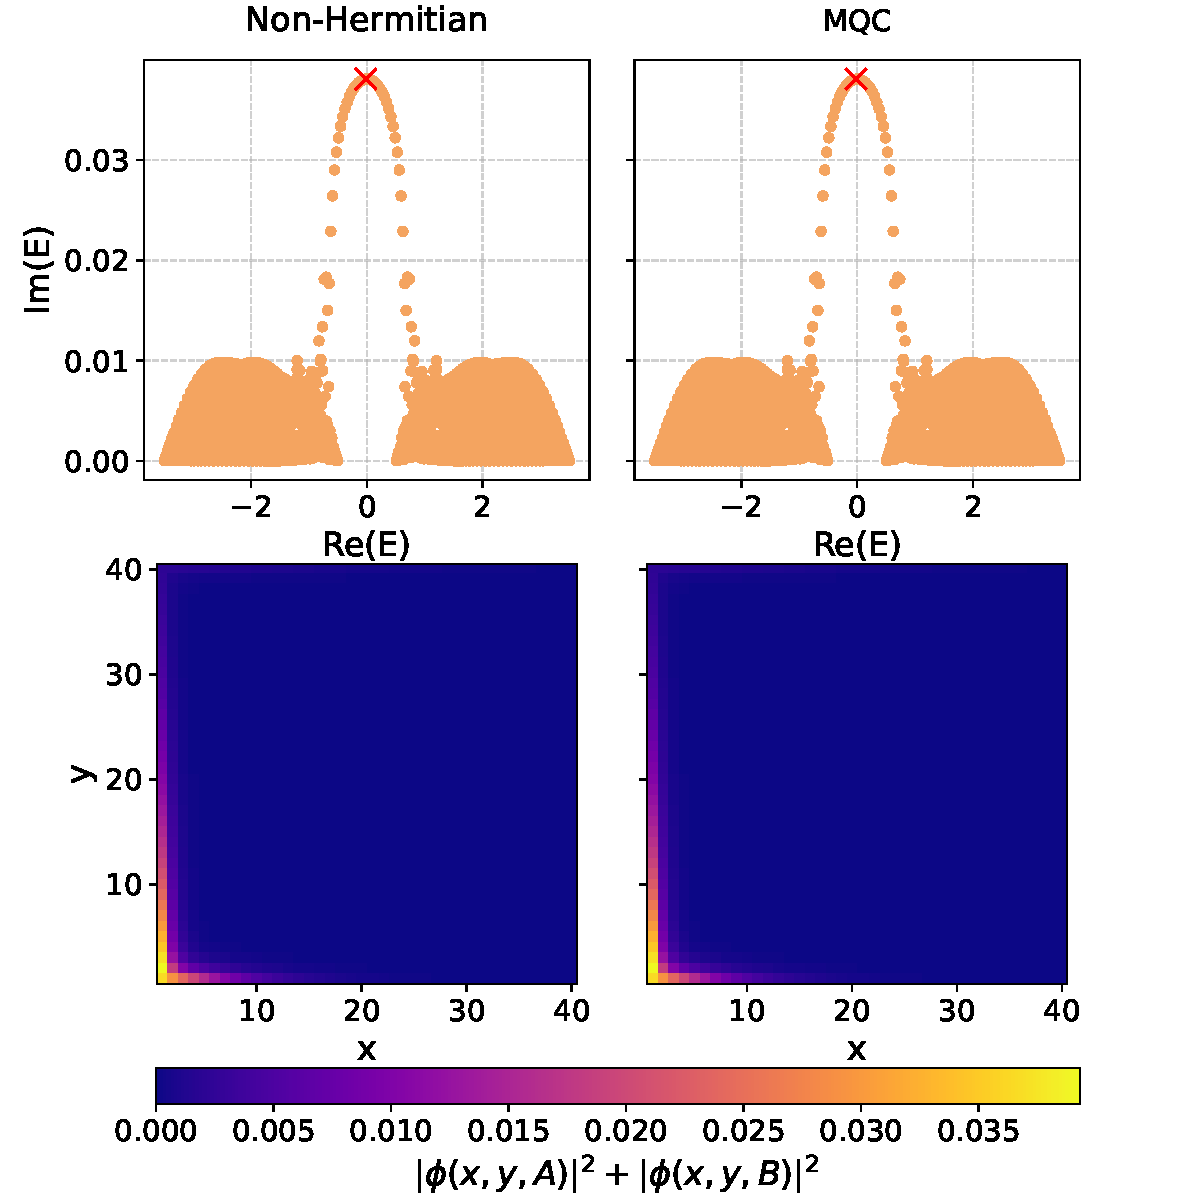
\includegraphics[width=1.\linewidth]{Picture/SingleExcitation_Comp.pdf}
		\caption{双激发子空间中能谱和本征态对比，$\gamma=-0.2$的非厄米耗散$\hat{H}_{\text{im}}$作用于$y=1$边界的元胞。(a) 在不存在相互作用和(b) 存在相互作用时的能谱。(c) 在不存在相互作用和(d) 存在相互作用时本征态的模方，其能量在(a)和(b)中用橘色十字表示。(e) (c)中本征态在各个格点的粒子数平均数，该态是多粒子的chiral skin mode。(f) (d)中本征态在各个格点的粒子数平均数，该态是NHMBL。系统尺寸为$L_x=L_y=9$，在位能为$u=-1.5$。}
		\label{fig:13}
	\end{figure} %label from y=1 and x=1?
	% 放intra的，以及不是拓扑绝缘体的时候，还有耗散并不加在边界的时候。在机理解释的时候，以及能谱的时候可以说一下anti-PT symmetry. 

	% \begin{figure*}[h]
	% 	\centering
	% 	\begin{minipage}[b]{0.49\linewidth}
	% 		\centering
	% 		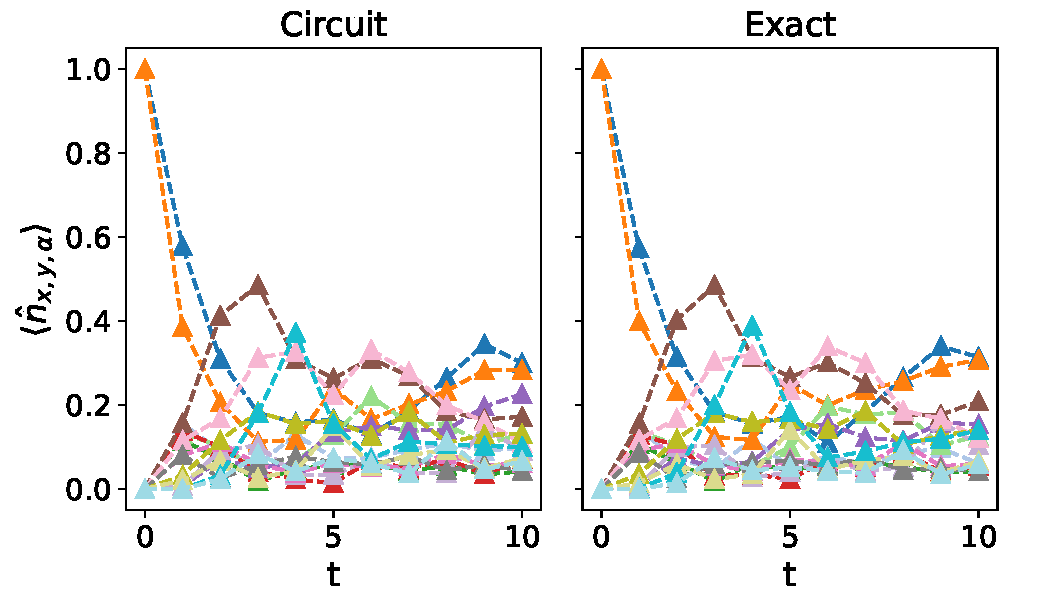
\includegraphics[width=\linewidth]{Picture/CircuitEvolve_ManyBody.pdf}
	% 		\caption{Single Excitation}
	% 		\label{fig:08}
	% 	\end{minipage}
	% 	\hfill
	% 	\begin{minipage}[b]{0.49\linewidth}
	% 		\centering
	% 		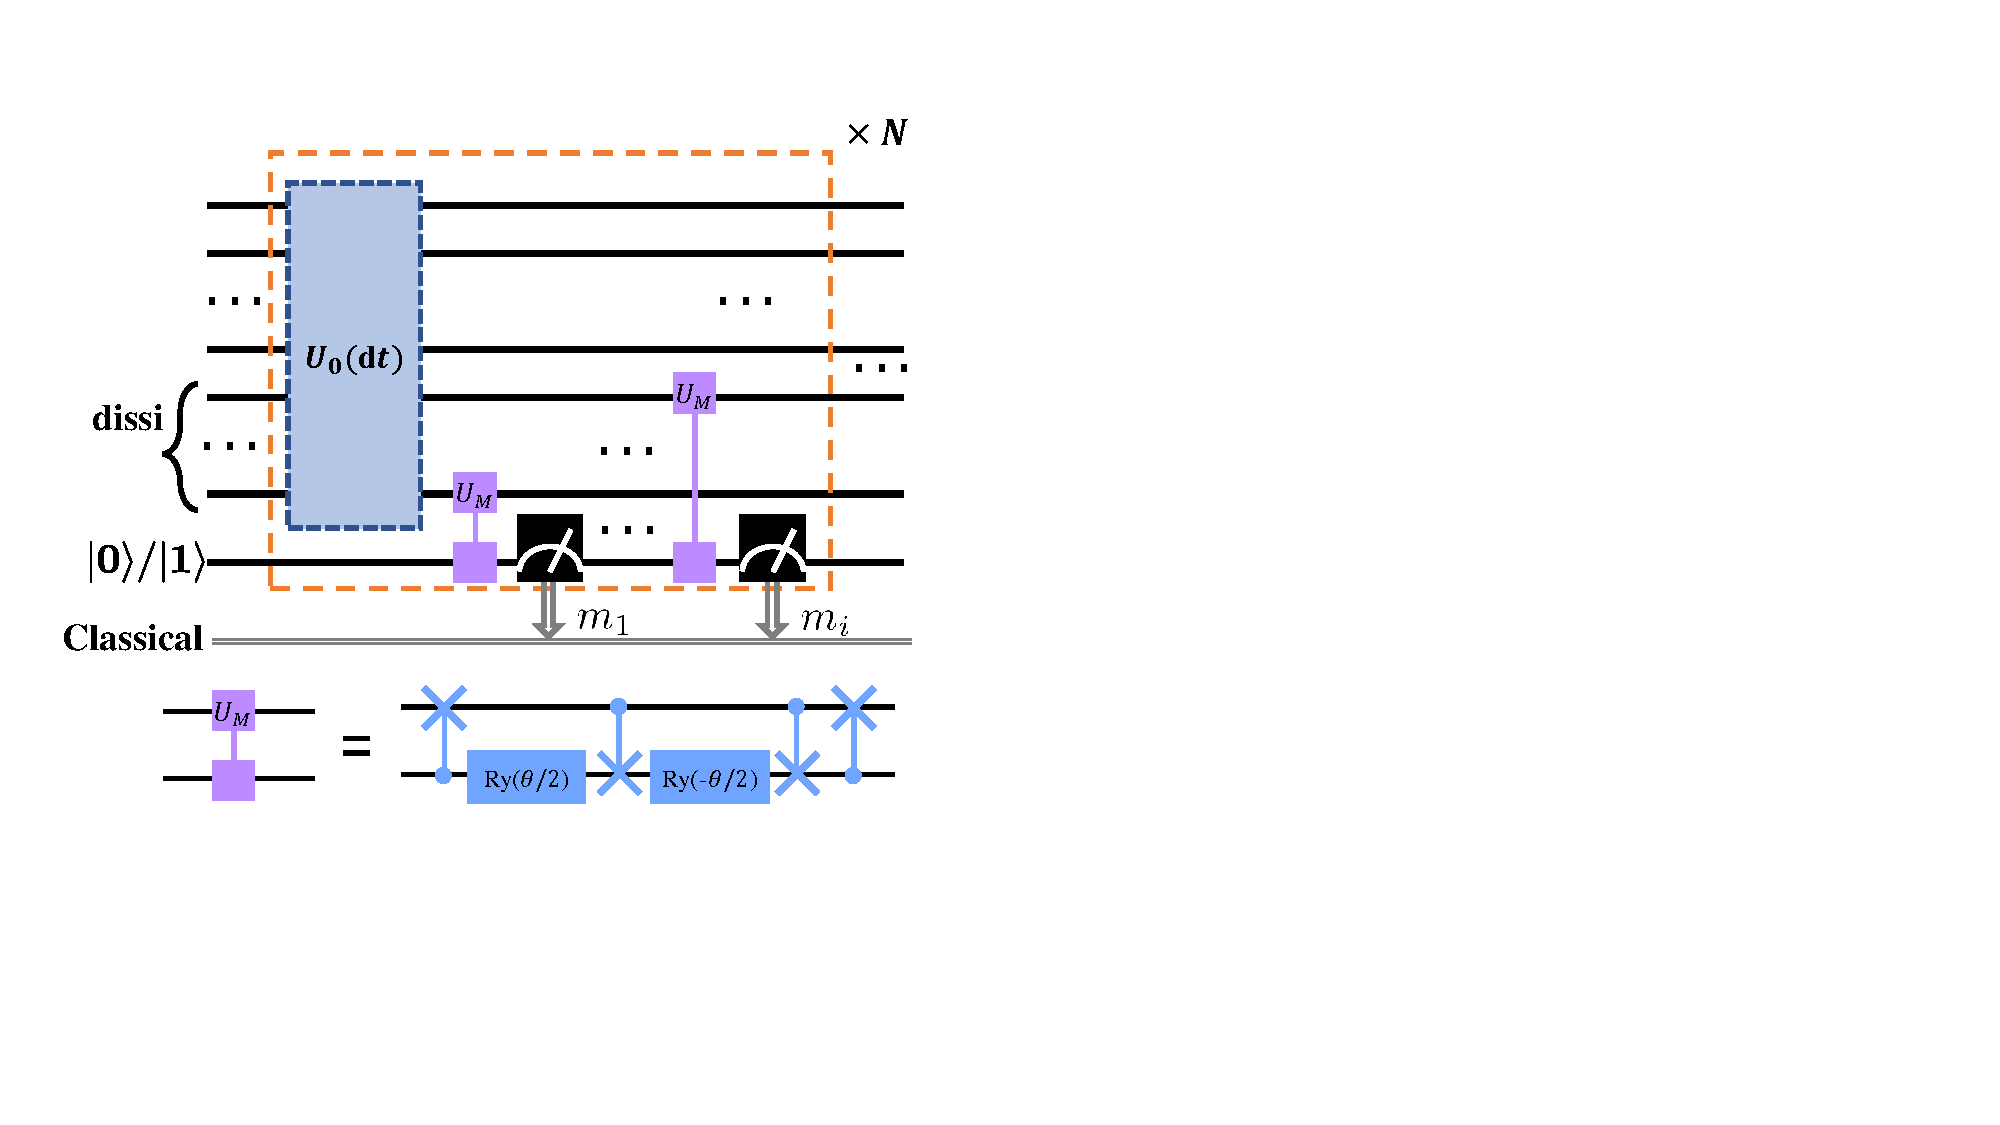
\includegraphics[width=\linewidth]{Picture/Circuit_Experiment.pdf}
	% 		\caption{Monitored quantum circuits.}
	% 		\label{fig:07}
	% 	\end{minipage}
	% \end{figure*}

	\section{Method~\label{sec:method}}
	\subsection{Implementation the gain/loss Hamiltonian in monitored quantum circuits}
	% 不用管那个，因为mqc本身实现非厄米，nc又不是第一篇
	% 就按照我们自己的来写。最后落脚在chiral skin就行

	In this part, we show how to realize the time evolution of the gain/loss non-Hermitian Hamiltonian. The non-Hermitian Hamiltonian $\hat{H}_{\text{non}}$ consists of Hermitian part $\hat{H}_0$, such as the Hamiltonian of QWZ model, and non-Hermitian part $\hat{H}_{\text{im}}$.
	\begin{equation}
		\hat{H}_{\text{non}} = \hat{H}_0 +\hat{H}_{\text{im}}. \label{eq:non-hermitian}
	\end{equation}
	The non-Hermitian part $\hat{H}_{\text{im}}$ is the sum of gain/loss energy on each site, which holds imaginary onsite energy, such as $\hat{H}_{\text{im}} = \sum_{i\in \text{dissi}} -\mathrm{i}\tilde{\gamma} \hat{c}_i^{\dagger} \hat{c}_i$ for dissipative energy. 
	%The time evolution of the Hermitian part. 
	To realize the time evolution of non-Hermitian Hamiltonian with time \textit{t}, labeled as $U(t) = e^{-\mathrm{i}(\hat{H}_0+\hat{H}_{\text{im}})t}$, we first construct $U(\mathrm{d} t)$ and  
	% The condition of dt is defined below.
	$U(t)$ is constructed by repeatedly acting $U(\mathrm{d} t)$.
	We define $\mathrm{d} t$ as the measurement interval, which is the unitary evolution time between measurements in two layers.
	
	To realize $U(\mathrm{d} t)$, we first act the time evolution of $\hat{H}_{0}$, labeled  as $U_0(\mathrm{d}t)=e^{-\mathrm{i}\hat{H}_0 \mathrm{d} t}$, and then local generalized measurements on the gain/loss sites, see Fig.~\ref{fig:01}.
	%In addition, we should emphasize that this projective measurement can be cancelled in each layer and a projective measurement on the ancilla at the end of the whole process is enough.
	% P0 at the end of the whole process is enough, the provement or statement should be added
	The generalized measurements are defined as a set of Kraus operators $\{M_{i,\beta},\beta=0,\pm \}$, which are a completely positive trace-preserving map. Without any postselection, the map is defined as
	$\varepsilon(\rho) = \sum_{\beta} M_{i, \beta} \rho M_{i, \beta}^{\dagger}$, and $\rho$ is density matrix of the fermionic system.
	The generalized measurements on the ith site are defined as
	\begin{align}
		&M_{i,\pm} = \sqrt{\frac{1}{2+(e^{\gamma \mathrm{d} t} - e^{-\gamma \mathrm{d} t})^2}} (1 + (e^{\pm \gamma \mathrm{d} t}-1) \hat{c}_i^{\dagger} \hat{c}_i),\\
		&M_{i,0} = \sqrt{\frac{(e^{\gamma \mathrm{d} t} - e^{-\gamma \mathrm{d} t})^2}{2+(e^{\gamma \mathrm{d} t} - e^{-\gamma \mathrm{d} t})^2}} c_i^{\dagger},
	\end{align}
	which satisfy the trace-preserving condition $\sum_{\beta} M_{i,\beta}^{\dagger} M_{i,\beta}=\mathrm{I}$. 
	Note that measurement interval $\mathrm{d}t$ is a parameter in the generalized measurements. 
	The generalized measurements can also be denoted as 
	\begin{align}
		&M_{i,\pm} = \sqrt{\frac{1}{2+(e^{\gamma \mathrm{d} t} - e^{-\gamma \mathrm{d} t})^2}} e^{\pm\gamma \hat{c}_i^{\dagger} \hat{c}_i\mathrm{d} t},\\
		&M_{i,0} = \sqrt{\frac{(e^{\gamma \mathrm{d} t} - e^{-\gamma \mathrm{d} t})^2}{2+(e^{\gamma \mathrm{d} t} - e^{-\gamma \mathrm{d} t})^2}} c_i^{\dagger}.
	\end{align}	
	Although not all operations can be implemented, the measurements above can be realized through projection measurements in an enlarged Hilbert space, as guaranteed by the Naimark's theorem~\cite{coecke2008povms,nielsen2001quantum}. As a result, our scheme can be implemented with current experimental techniques through the introduction of auxiliary qubits.
	The dissipative non-Hermitian Hamiltonian with onsite loss $-\mathrm{i}\gamma$ can be realized through postselecting $M_{i,-}$, while the non-Hermitian Hamiltonian with onsite gain $\mathrm{i}\gamma$ can be realized through postselecting $M_{i,+}$.
	% under what condition, it is a projective measurement!(no) Explain our measurement. 
	
	Our measurement scheme postselects the outcome of $M_{i,-}$ for dissipative non-Hermitian, which maps the state $\vert \psi \rangle$ to $M_{i,-} \vert \psi \rangle/\Vert M_{i,-} \vert \psi \rangle \Vert$ with a probability of $\Vert M_{i,-} \vert \psi \rangle \Vert^2$. 
	%If the Hermitian part $\hat{H}_0$ and the non-Hermitian part $\hat{H}_{\text{im}}$ are not commutative, 
	The parameter of measurements should satisfy $\gamma \mathrm{d} t \ll 1$. To postselect the $M_{i,-}$ over n measurements, we need roughly to perform  $2^n$ experiments. 
	% how to realize the POVM, add some citations.
	%Unitary evolution of $\hat{H}_0$ followed by postselective measurements on all dissipative sites is described as $E=(\prod_{i\in \text{dissi}} M_{i,-}) U_{0}(\mathrm{d} t),U_{0}(\mathrm{d}t)=e^{-\mathrm{i}\hat{H}_0 \mathrm{d}t}$. 
	The whole evolution process is to first perform the unitary evolution of $\hat{H}_0$ on all sites and then the generalized measurements on all dissipative sites. It is described as $E=(\prod_{i\in \text{dissi}} M_{i,-}) U_{0}(\mathrm{d} t),U_{0}(\mathrm{d}t)=e^{-\mathrm{i}\hat{H}_0 \mathrm{d}t}$.
	Instead of performing all measurements on gain/loss sites, our scheme performs the measurement on each gain/loss site with a classical probability $p\in(0,1]$.
	%, see Fig.~\ref{fig:monitoredquantumcircuit}(a). 
	Then we obtain a probabilistic quantum circuit operator, and the process of performing it on an initial state $\vert \psi \rangle$ is described by
	\begin{equation}
		\frac{E(p,r) \vert \psi \rangle}{\Vert E(p,r) \vert \psi \rangle \Vert} = \frac{(\prod_j M_{j,-}^{r_j}) \cdot U_0(\mathrm{d}t)}{\Vert (\prod_j M_{j,-}^{r_j}) \cdot U_0(\mathrm{d}t) \vert \psi \rangle \Vert} \vert \psi \rangle,
	\end{equation}
	where $U_0(\mathrm{d} t) = e^{-\mathrm{i}\hat{H}_0 \mathrm{d} t}$ and $r_j$ = 0 or 1 with a probability of $1-p$ and $p$, respectively. So $N$-layer MQC with a probability of $p$ is defined as
	\begin{equation}
		E_N(p,\{r\}) = E(p, r_N) \circ E(p, r_{N-1}) \circ \cdots \circ E(p, r_1).
	\end{equation}
	% define effective Hamiltonian
	The effective Hamiltonian $\hat{H}_{\text{eff}}^{(N)}$ of this $N$-layer MQC is defined as
	\begin{equation}
		e^{-\mathrm{i}\hat{H}_{\text{eff}}^{(N)} N \mathrm{d} t} = E_N(p,\{r\}). \label{eq:H_scheme1}
	\end{equation}
	\iffalse
	We define the effective Hamiltonian of a finite \textit{N}-layer quantum circuit as 
	\begin{align}
		\hat{H}^{(N)}_{\text{eff}} (p,\mathrm{d}t, \{s\}) &= \frac{i}{N\mathrm{d}t} \log{E_N(p, \{r\})} \notag\\
		&= \frac{i}{N\mathrm{d}t} \sum_{i=1}^N \log{E(p,r_i)}. \label{eq:EffectiveH}
	\end{align}\
	\fi
	
	%Take Fig.~\ref{fig:monitoredquantumcircuit}(c) as an example, the non-Hermitian Hamiltonian is defined on a square lattice, where the red points indicate the unit cells and the red points in the blue rectangle indicate the gain (loss) unit cells with $\mathrm{i}\gamma \sigma_0$ ($-\mathrm{i}\gamma \sigma_0$ ) imaginary onsite energy, where $\sigma_0$ is the identity matrix. The first scheme to realize this non-Hermitian Hamiltonian is to apply unitary evolution $U_0(\mathrm{d}t)$ of the Hermitian part. And then each generalized measurement in the blue rectangle is applied with probability $p$. The above sequence is one layer of the quantum circuit, and $N$-layer quantum circuit can realize $N\mathrm{d}t$ time evolution of the non-Hermitian Hamiltonian, as depicted in Fig.~\ref{fig:monitoredquantumcircuit}(a). 

	% \subsection{The relationship between measurement-induced topology and non-Hermitian topology}
	\subsection{The relationship between the MQC and non-Hermitian Hamiltonian}
	
	% We need to show when T is infinite, Floquet-Magnus expansion, Pi M = exp(). Then gives out the error. While the second scheme does not.
	In this part, we take the dissipative non-Hermitian Hamiltonian as an example. When $p=1$, the circuit of the first scheme is periodic and we get the Floquet Hamiltonian $\hat{H}_{F}$, which captures the dynamic at time $m \mathrm{d}t$ ($m$ is an integer). 
	The measurement operator is $\prod_{i\in \text{dissi}} M_{i, -} \propto e^{-i\sum_{i\in \text{dissi}} \gamma \hat{c}_i^{\dagger} \hat{c}_i \mathrm{d}t}$. In the high frequency limit, $\nu\mathrm{d}t \ll 1$ ($\nu$ is the typical energy scale, such as $\tilde{\gamma}$), the Floquet Hamiltonian (to leading order in inverse frequency) equals to~\cite{bukov2015universal,RN694}
	\begin{equation}
		\hat{H}_F = \hat{H}_0 + \sum_{i\in \text{dissi} } (-\mathrm{i}\gamma \hat{c}_i^{\dagger} \hat{c}_i) + \mathcal{O}(\nu \mathrm{d} t).
	\end{equation}
	So the dynamics of the exponential long time($\propto e^{1/(\nu \mathrm{d} t)}$) is captured by the Floquet Hamiltonian $\hat{H}_F$~\cite{RN1228}. The Floquet Hamiltonian here is used to analytically explain that the effective Hamiltonian of the circuit is the non-Hermitian Hamiltonian expected and the error of our simulation of the non-Hermitian Hamiltonian is $\mathcal{O}(\nu \mathrm{d} t)$.
	The periodic condition of time is violated when $p\neq 1$. 
	
	%In the ideal case, the measurement $M_{i,-}^{r_i}$ can be viewed as that the measurement $M_{i,-}$ is imposed with probability $p$, and no operations are imposed with probability $1-p$. 
	When $p\neq1$, the quantum circuit can also be understood from the perspective of Trotter expansion but our schemes require fewer measurements than the Trotter expansion. In our scheme, the measurement $M_{i,-}$ is imposed with probability $p$ and no operations are imposed with probability $1-p$ in each layer. When $\gamma \mathrm{d}t\ll 1$ is satisfied, the effective operation $M_{i,-}^{r_i}$ is $e^{-p \gamma \hat{c}_i^{\dagger} \hat{c}_i \mathrm{d}t} $. To clarify it and its error, we define the effective Hamiltonian of a finite \textit{N}-layer quantum circuit as 
	\begin{align}
		\hat{H}^{(N)}_{\text{eff}} (p,\mathrm{d}t, \{s\}) &= \frac{\mathrm{i}}{N\mathrm{d}t} \log{E_N(p, \{r\})} \notag\\
		&= \frac{\mathrm{i}}{N\mathrm{d}t} \sum_{i=1}^N \log{E(p,r_i)}.
	\end{align}
	The total effective Hamiltonian $\hat{H}^{(N)}_{\text{eff}}$ is the average of the effective Hamiltonian of each layer, which imposes the generalized measurements with probability $p$. According to the central limit theorem, the deviations decrease as $1/\sqrt{N}$ when we increase the layer of MQC. In this limit, the effective 
	% Here the deviation means every judge parameter to judge the difference between the target and real, such as norm, falls off as 1/$\sqrt{N}$.
	Hamiltonian $\hat{H}^{(N)}_{\text{eff}}$ of \textit{N}-layer quantum circuit is 
	\begin{equation}
		\hat{H}^{(N)}_{\text{eff}} = \hat{H}_0 + \sum_{i\in \text{dissi} } (-\mathrm{i} p\gamma \hat{c}_i^{\dagger} \hat{c}_i) + \mathcal{O}(\nu\mathrm{d} t) + \mathcal{O}(1/\sqrt{N}).
	\end{equation}
	At large $N$, we can replace the probabilistic quantum circuit with $p$ and $\gamma$ with a deterministic quantum circuit with $\gamma_{\text{eff}} = p \gamma$. The dynamic of the probabilistic quantum circuit is equivalent to that of the deterministic quantum circuits. According to the discussion above, $\hat{H}^{(N)}_{\text{eff}}$ is the non-Hermitian Hamiltonian with gain or loss onsite energy. 
	% Why the dynamic of the corner state can be captured by a small N?
	
	% 暂时不要第二种方案。
	% Moreover, the second scheme can generate the effective Hamiltonian without any error
	% \begin{equation}
	% 	\hat{H}_{\text{eff}} = \hat{H}_0 + \sum_{i\in \text{dissi} } (-ip\gamma \hat{c}_i^{\dagger} \hat{c}_i).
	% \end{equation}
	% Because the Hermitian part and the non-Hermitian part are commutative and the measurement $M_{i,-}$ can generate the imaginary onsite energy without any error. If $\mathrm{d}t$ is small, it can increase the success probability and shorten the unitary evolution time.
	
	% According to the discussion above, $\hat{H}^{(N)}_{\text{eff}}$% and $\hat{H}_{\text{eff}}$ 
	% is the non-Hermitian Hamiltonian with gain or loss onsite energy. 
	%According to the discussion above, $\hat{H}_0 + \sum_{i\in \text{dissi} } (-ip\gamma \hat{c}_i^{\dagger} \hat{c}_i)$ in the effective Hamiltonian $\hat{H}^{(N)}_{\text{eff}}$ and $\hat{H}_{\text{eff}}$ is the non-Hermitian Hamiltonian $\hat{H}_{\text{non}}$ with dissipative sites. 

	\subsection{Experimental Realizations}
	The non-Hermitian term can be realized through the generalized measurements. The realization of generalized measurements $\{M_{i,\beta}, \beta=\pm,0\}$ is diffcult. However, measurement $M_{i,+}$ and measurement $M_{i,-}$ can be realized though one ancilla qubit. We first act a two-qubit unitary gates to the qubit and the ancilla qubit, which is
	\begin{equation}
		U_{\text{M}} = \begin{pmatrix}
		  1 & 0 & 0 & 0\\
		  0 & e^{-\gamma \dif t} & \sqrt{1-e^{-2 \gamma \dif t}} & 0\\
		  0 & -\sqrt{1-e^{-2 \gamma \dif t}} & e^{-\gamma \dif t} & 0\\
		  0 & 0 & 0 & 1
		\end{pmatrix}.
	\end{equation}
	If the ancilla qubit is prepared on state $\ket{0}$($\ket{1}$), the measurement $M_{i,-}$($M_{i,+}$) can be realized when the measurement on the ancilla qubit gives $\ket{0}$ ($\ket{1}$) results. Through the two-qubit gates and the measurement on the ancilla qubit, we can realize the time evolution $e^{-\mathrm{i} (\pm \mathrm{i} \hat{c}_i^{\dagger}\hat{c}_i) \mathrm{d}t}$ of non-Hermitian Hamitltonian.
	% 最后给出后选择概率，说明比较容易实现。可以提一下Zeno效应吗？

	% \subsection{Chiral skin effect with many-body interaction}
	% We consider about the Qi-Wu-Zhang model with Hamiltonian
	% \begin{align}
	% 	\hat{H}_{\text{QWZ}} &=  \sum_{m_{x}=1}^{N_{x}-1} \sum_{m_{y}=1}^{N_{y}}\left(\hat{c}_{m_{x}+1, m_{y}}^{\dagger} \hat{c}_{m_{x}, m_{y}} \otimes \frac{\hat{\sigma}_{z}+i \hat{\sigma}_{x}}{2}+\mathrm{H.c.}\right) \notag\\
	% 	& +\sum_{m_{x}=1}^{N_{x}} \sum_{m_{y}=1}^{N_{y}-1}\left(\hat{c}_{m_{x}, m_{y}+1}^{\dagger} \hat{c}_{m_{x}, m_{y}} \otimes \frac{\hat{\sigma}_{z}+i \hat{\sigma}_{y}}{2}+\mathrm{H.c.}\right) \notag\\
	% 	& +u \sum_{m_{x}=1}^{N_{x}} \sum_{m_{y}=1}^{N_{y}} \hat{c}_{m_{x}, m_{y}}^{\dagger} \hat{c}_{m_{x}, m_{y}} \otimes \hat{\sigma}_{z},
	% \end{align}
	% where $\hat{c}_{m_{x}, m_{y}}^{\dagger}$ ($\hat{c}_{m_{x}, m_{y}}$) is the creation (annihilation) operators at site $(m_x,m_y)$, and each unit cell has two sites. 
	
	% In order to study the chiral skin effect in presence of many-body interaction, we consider the following many-body interaction
	% \begin{widetext}
	% 	\begin{align}
	% 		\hat{H}_{\text{inter}} = &\sum_{{x}=1}^{L_{x}-1} \sum_{{y}=1}^{L_{y}}  U_{\text{inter}} \left(\hat{n}_{{x}, {y}, A}+\hat{n}_{{x}, {y}, B}\right) \left(\hat{n}_{{x}+1, {y}, A}+\hat{n}_{{x}+1, {y}, B}\right)\\
	% 		& + 
	% 		\sum_{{x}=1}^{L_{x}} \sum_{{y}=1}^{L_{y}-1}  U_{\text{inter}} \left(\hat{n}_{{x}, {y}, A}+\hat{n}_{{x}, m_y, B}\right) \left(\hat{n}_{{x}, {y}+1, A}+\hat{n}_{{x}, {y}+1, B}\right),\\
	% 		\hat{H}_{\text{intra}} &= \sum_{{x}=1}^{L_{x}-1} \sum_{{y}=1}^{L_{y}}  U_{\text{intra}} \hat{n}_{{x}, {y}, A} \hat{n}_{{x}, {y}, B}.
	% 	\end{align}
	% \end{widetext}
	% where $\hat{n}_{{x}, {y}, A}$ ($\hat{n}_{{x}, {y}, B}$) is the number operator at sublattice $A$ ($B$) of unit cell $({x}, {y})$. And $U_{\text{inter}}$ and $U_{\text{intra}}$ is interaction strength. 
	% % 可以加以一段为什么考虑这两个，有理就可以。
	
	\appendix

	\section{The $\mathcal{P}_{x,y,\alpha}$ at different time and interaction strength~\label{sec:AllP}}

	我们研究了在不同时间和相互作用强度$U_{\text{inter}}$下在各个格点处$\mathcal{P}_{x,y,\alpha}$的值。我们分别计算了在哈密顿量$\hat{H}_{\text{QWZ}}+\hat{H}_{\text{inter}}$和$\hat{H}_{\text{QWZ}}+\hat{H}_{\text{inter}}+\hat{H}_{\text{im}}$演化下在时间$t=20$和$t=60$时刻$\mathcal{P}_{x,y,\alpha}$。结果表明在只存在多体相互作用的时候，所有格点的$\mathcal{P}_{x,y,\alpha}$都随相互作用强度$\vert U_{\text{inter}} \vert$的增加而减小，这表明随着相互作用强度的增加，量子态更趋向于演化向非局域的量子态。而在存在非厄米的时候，部分格点的$\mathcal{P}_{x,y,\alpha}$同样随相互作用强度的增加而减小。但是在部分格点处的$\mathcal{P}_{x,y,\alpha}$随相互作用的增加先减小后增加。这是由于NHMBL，导致从任意格点出发的粒子最后都会演化到局域化的量子态，从而被探测到。且上面的现象随着时间的增加更加明显，因为此时更加趋向于稳态。

	\begin{figure}[h]
		\centering
		%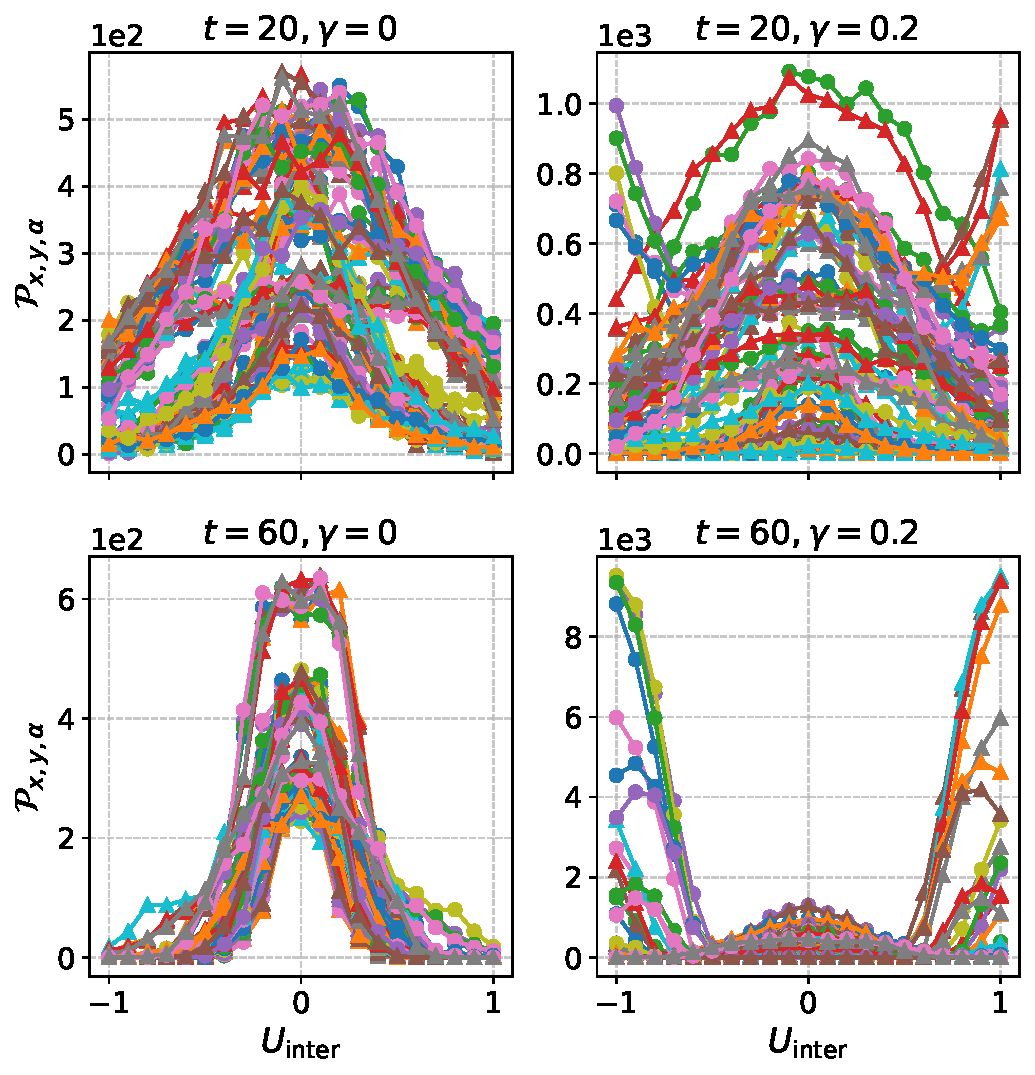
\includegraphics[width=1.\linewidth]{Picture/SI/SI_Popu_Interaction.pdf}
		\begin{overpic}[width=1.0\linewidth]{Picture/SI/SI_Popu_Interaction.pdf}
			\put(3,98){(a)}
			\put(50,98){(b)}
			\put(3,50){(c)}
			\put(50,50){(d)}
			% \put(49,54){(d)}
		\end{overpic}
		\caption{在时间$t=20$和$t=60$时，不同相互作用强度下的$\mathcal{P}_{x,y,\alpha}$。(a) 在时间$t=20$，不存在非厄米增益的多体哈密顿量。(b) 在时间$t=20$，存在$\gamma=0.2$的$\hat{H}_{\text{im}}$的多体非厄米哈密顿量。(c) 在时间$t=60$，不存在非厄米增益的多体哈密顿量。(d) 在时间$t=60$，存在$\gamma=0.2$的$\hat{H}_{\text{im}}$的多体非厄米哈密顿量。增益作用于$y=1$元胞。系统尺寸为$L_x=L_y=7$，在位能为$u=-1.5$。选取的随机初始量子态数目为$N_{\text{samp}}=10^4$。}
		\label{fig02}
	\end{figure}

	\section{Non-Hermitian Many-Body Localization: Robustness, Existence Beyond Edge States\label{sec:NHMBL}}

	\subsection{Robust to the localtion of dissipative site}

	% Unlike chiral skin mode, the chiral skin mode emergences when the dissipative sites are placed on the boundary of the lattice. The chiral skin mode emergence when edge state of topological insulator posses a finite lifetime. 
	chiral skin mode是在耗散元胞位于晶格边界时出现的。当拓扑绝缘体的边缘态具有有限的寿命时，手性皮肤模式会出现。
	% beyond topological transition.
	在这里，我们阐明NHMBL并非简单的多体chiral skin effect。实际上当系统的体中存在增益的时候，NHMBL依然存在，且量子态并不会局域化在系统边界。我们考虑一个$L_x=L_y=9$的二维系统，且增益施加在$y=3$的所有元胞上，包含和不包含多体相互作用的非厄米哈密顿量的能谱和本征态分别展示在Fig.~\ref{fig:10}的第一列和第二列。Fig.~\ref{fig:10}的结果表明，在没有多体相互作用的情况下，因非厄米增益未作用于边缘态，所以此时并未出现局域化的chiral skin mode，虚本征值最大的本征态变为了bulk state，如图Fig.~\ref{fig:10} (e)所示。当存在多体相互作用时，由于相互作用引起的能级差以及非厄米pumping的共同作用，NHMBL得以存在，并且此时量子态局域化于$y=3$元胞的$B$子晶格。
	\begin{figure}[h]
		\centering
		\begin{overpic}[width=1.0\linewidth]{Picture/SI/SI_TwoExcitationSpectrum_NotEdge.pdf}
			\put(4,97){(a)}
			\put(42,97){(b)}
			% \put(7,54){(c)}
			\put(4,62){(c)}
			\put(42,62){(d)}
			\put(4,26){(e)}
			\put(42,26){(f)}
		\end{overpic}
		%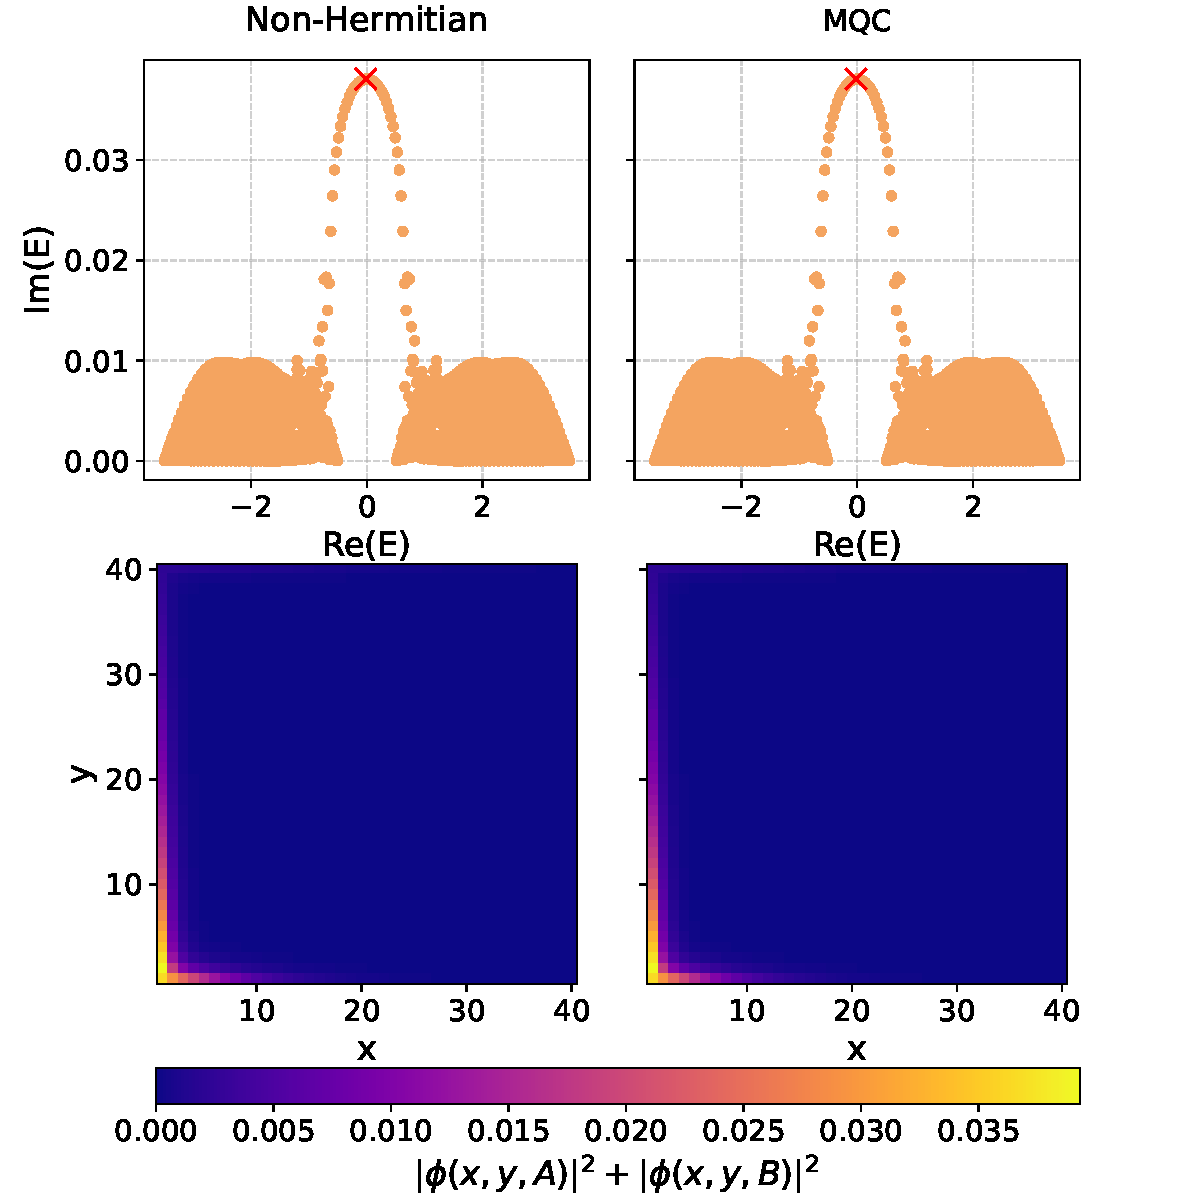
\includegraphics[width=1.\linewidth]{Picture/SingleExcitation_Comp.pdf}
		\caption{双激发子空间中能谱和本征态对比，$\gamma=0.2$的非厄米增益$\hat{H}_{\text{im}}$作用于$y=3$边界的元胞。(a) 在不存在相互作用和(b) 存在相互作用时的能谱。(c) 在不存在相互作用和(d) 存在相互作用时本征态的模方，其能量在(a)和(b)中用橘色十字表示。(e) (c)中本征态在各个格点的粒子数平均数，该态是多粒子的chiral skin mode。(f) (d)中本征态在各个格点的粒子数平均数，该态是NHMBL。系统尺寸为$L_x=L_y=9$，在位能为$u=-1.5$。}
		\label{fig:10}
	\end{figure} %label from y=1 and x=1?

	\subsection{The NHMBL exists even when there is no edge state}

	由于QWZ模型当$-2<u<0$和$0<u<2$时，模型表现为拓扑绝缘体并存在边缘态。然而，当$u=2.1$时，QWZ模型变为拓扑平庸的绝缘体，此时不再存在edge state。我们考虑对一个拓扑平庸的绝缘体的边界施加增益，并观察是否会出现chiral skin mode和NHMBL。根据chiral skin effect的理论，对仅存在bulk state的系统施加增益并不会导致chiral skin mode，如Fig.~\ref{fig:10}(e)所示。然而，当我们在没有边缘态的拓扑绝缘体中施加增益和多体相互作用时，NHMBL会出现(Fig.~\ref{fig:10}(f))，这是因为非厄米pumping和多体相互作用引起的能级差仍然存在。因此它们的共同作用导致了NHMBL的出现。由此可见，NHMBL的存在并不依赖于厄米哈密顿量是否为拓扑绝缘体，也不依赖于增益是否作用于边缘态。
	% 对于增益和耗散是否存在对称性？存在，但是如何解释机理呢？从对称性来。
	% 增益和耗散是左矢和右矢的区别。
	\begin{figure}[h]
		\centering
		\begin{overpic}[width=1.0\linewidth]{Picture/SI/SI_TwoExcitationSpectrum_NotTopology.pdf}
			\put(4,97){(a)}
			\put(42,97){(b)}
			% \put(7,54){(c)}
			\put(4,62){(c)}
			\put(42,62){(d)}
			\put(4,26){(e)}
			\put(42,26){(f)}
		\end{overpic}
		%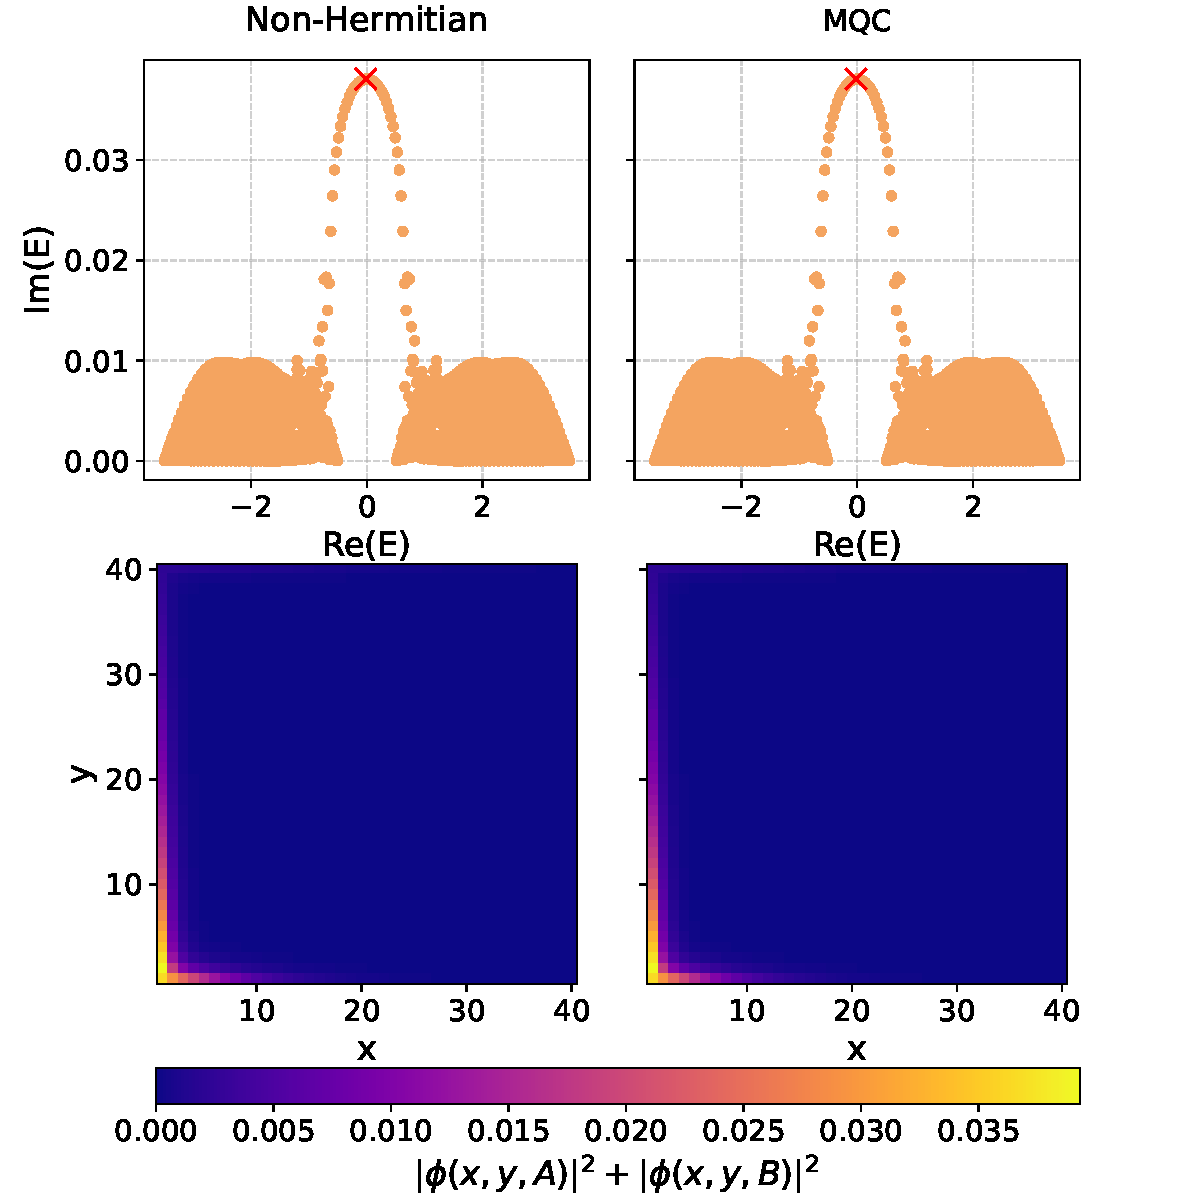
\includegraphics[width=1.\linewidth]{Picture/SingleExcitation_Comp.pdf}
		\caption{双激发子空间中能谱和本征态对比，$\gamma=0.2$的非厄米增益$\hat{H}_{\text{im}}$作用于$y=1$边界的元胞。(a) 在不存在相互作用和(b) 存在相互作用时的能谱。(c) 在不存在相互作用和(d) 存在相互作用时本征态的模方，其能量在(a)和(b)中用橘色十字表示。(e) (c)中本征态在各个格点的粒子数平均数，该态是多粒子的chiral skin mode。(f) (d)中本征态在各个格点的粒子数平均数，该态是NHMBL。系统尺寸为$L_x=L_y=9$，在位能为$u=-2.1$，此时QWZ模型是拓扑平庸的。 }
		\label{fig:11}
	\end{figure} %label from y=1 and x=1?
	
	\section{NHMBL with intra cell interaction\label{sec:NHMBL_intra}}

	在上述讨论中，我们主要考虑了多体相互作用$\hat{H}_{\text{inter}}$的情况。接下来，我们将探讨在其它类型的相互作用下，chiral skin mode和NHMBL是否存在。我们仅考虑元胞内$A$子格点和$B$子格点之间的粒子相互作用，形式为
	\begin{equation}
		\hat{H}_{\text{intra}} = \sum_{{x}=1}^{L_{x}-1} \sum_{{y}=1}^{L_{y}}  U_{\text{intra}} \hat{n}_{{x}, {y}, A} \hat{n}_{{x}, {y}, B}.
	\end{equation}
	我们考虑一个$L_x=L_y=9$的二维系统，且增益施加在$y=1$的所有元胞上。相应的结果展示在Fig.~\ref{fig:12}中。在相互作用强度$U_{\text{intra}}=1.0$的情况下，虽然本征态和本征值的形式与无多体相互作用时有所不同，利用粒子数算符描述多粒子的chiral skin mode仍然存在。这是因为多体相互作用$\hat{H}_{\text{intra}}$并未引入$\mathscr{H}_{\text{pump}}$空间中所有态与其它态之间的能级差，被pumping到该空间的粒子会有相当一部分通过跃迁的方式离开该空间，从而导致由于边缘态引起的chiral skin effect的出现，而不会导致NHMBL的出现。
	\begin{figure}[h]
		\centering
		\begin{overpic}[width=1.0\linewidth]{Picture/SI/SI_TwoExcitationSpectrum_intra.pdf}
			\put(4,97){(a)}
			\put(42,97){(b)}
			% \put(7,54){(c)}
			\put(4,62){(c)}
			\put(42,62){(d)}
			\put(4,26){(e)}
			\put(42,26){(f)}
		\end{overpic}
		%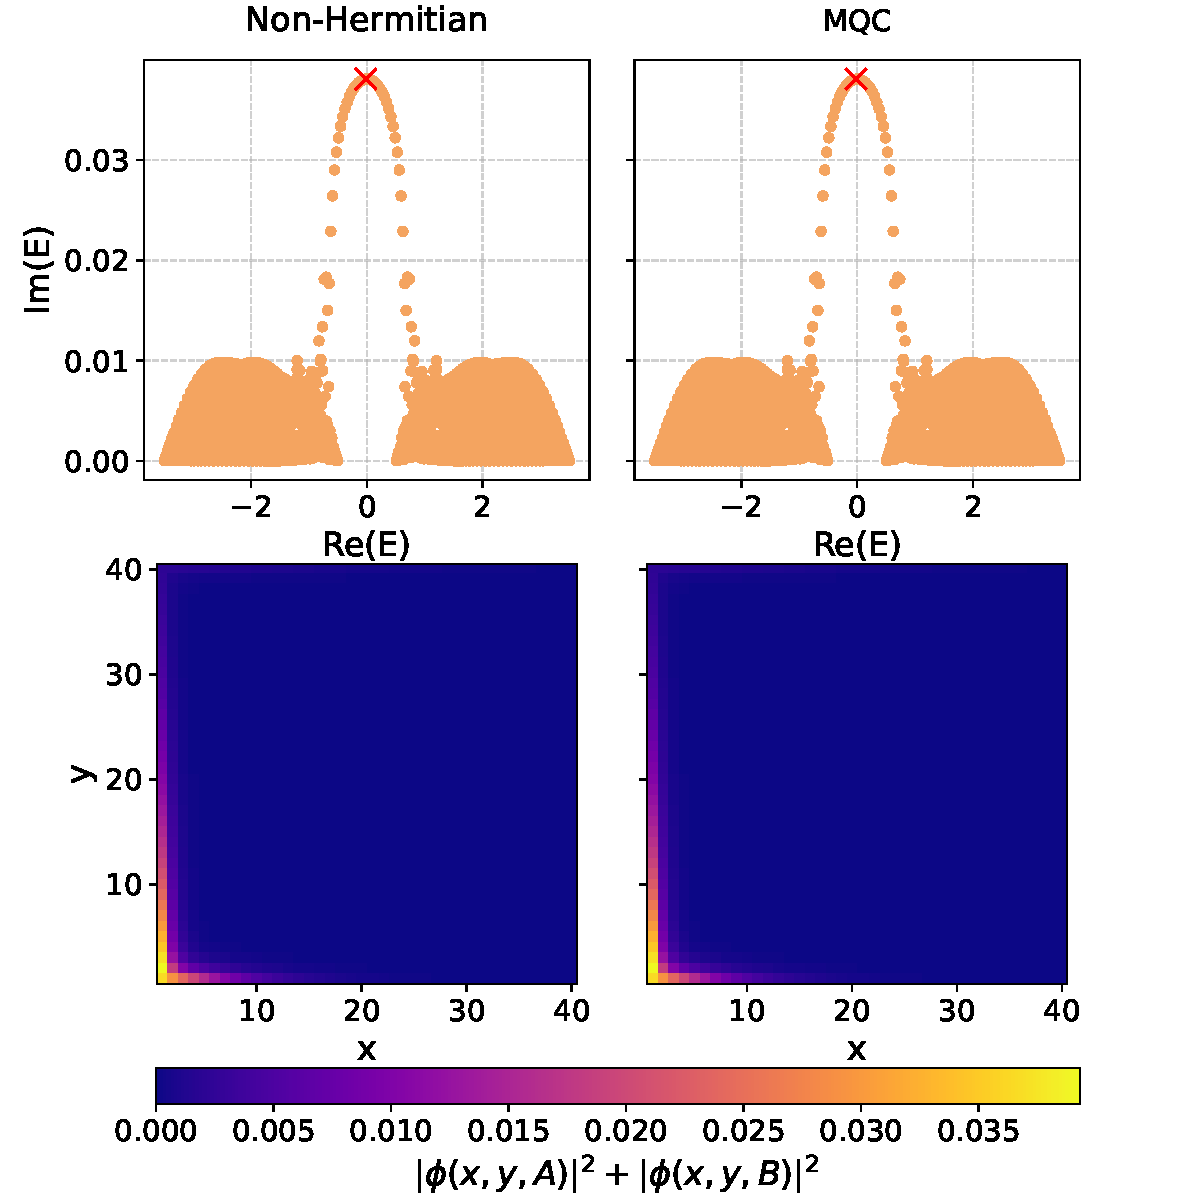
\includegraphics[width=1.\linewidth]{Picture/SingleExcitation_Comp.pdf}
		\caption{双激发子空间中能谱和本征态对比。$\gamma=0.2$的非厄米增益$\hat{H}_{\text{im}}$作用于$y=1$边界的元胞，多体相互作用为$\hat{H}_{\text{intra}}$。(a) 在不存在相互作用和(b) 存在相互作用时的能谱。(c) 在不存在相互作用和(d) 存在相互作用时本征态的模方，其能量在(a)和(b)中用橘色十字表示。(e) (c)中本征态在各个格点的粒子数平均数，该态是多粒子的chiral skin mode。(f) (d)中本征态在各个格点的粒子数平均数，该态是NHMBL。系统尺寸为$L_x=L_y=9$，在位能为$u=-1.5$。}
		\label{fig:12}
	\end{figure} %label from y=1 and x=1?

	\section{The evolution of 4 particles in the MQC~\label{sec:4Body_Evolve}}
	Here, we show the time evolution of multi-particles in the monitored quantum circuit. The comparisons between the results of the MQC and exact time-evolution are given in Fig.~\ref{fig:14}. 我们考虑一个$L_x=2,L_y=4$的二维晶格，耗散作用于$y=1$的边界上，相互作用部分为$U=1.0$的$\hat{H}_{\text{inter}}$，量子态初始的四个粒子分别位于元胞$(1,1)$和$(2,1)$的$A$格点和$B$格点。在随后的时间对各个格点测量$\langle \hat{n}_{x,y,\alpha}\rangle$，相应的结果如图Fig.~\ref{fig:14}。它们分别是通过我们的方案的MQC和精确的方法对增益非厄米多体哈密顿量的模拟结果。它们之间的吻合表明我们的方案的MQC仅通过一个辅助比特能够对在更多粒子激发的非厄米多体哈密顿量进行模拟。
	\begin{figure}[h]
		\centering
		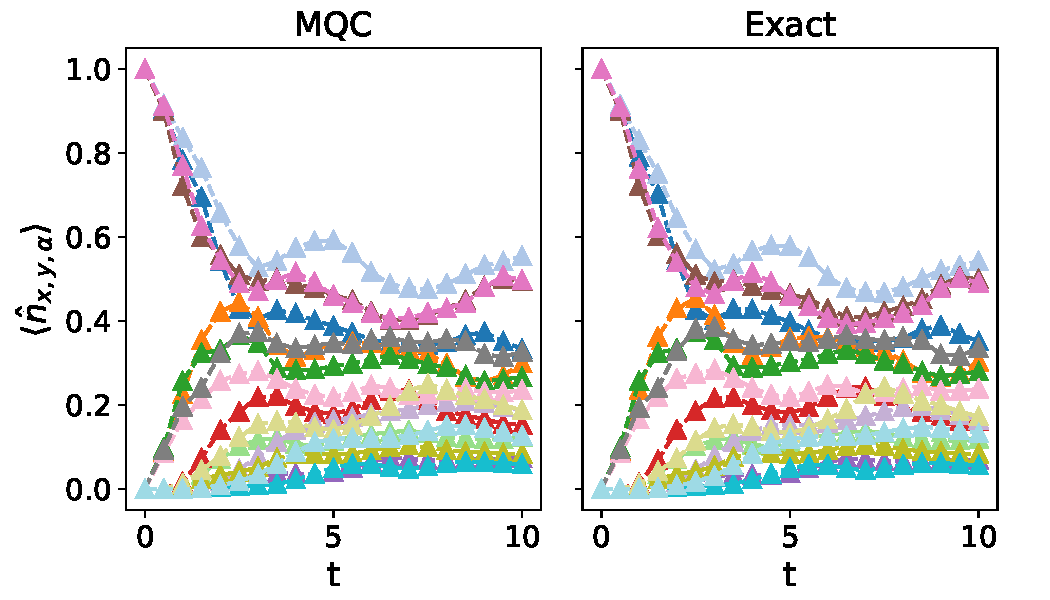
\includegraphics[width=1.\linewidth]{Picture/SI/SI_CircuitEvolve_4Body.pdf}
		\caption{从初始在元胞$(1,1)$和$(2,1)$的$A$子格点和$B$子格点各有一个粒子的四粒子态开始演化，在不同时间$t$不同格点的平均粒子数。分别是通过Fig.~\ref{fig:07}的量子线路和精确计算得到的。系统尺寸为$L_x=2,L_y=4$，相互作用强度为$U_{\text{inter}}=1.0$，非厄米参数为$\gamma=0.2$。受控量子线路参数为$\mathrm{d}t=0.1$,$N=50$}
		\label{fig:14}
	\end{figure}

	% If in two-column mode, this environment will change to single-column
	% format so that long equations can be displayed. Use
	% sparingly.
	%\begin{widetext}
	% put long equation here
	%\end{widetext}
	
	% figures should be put into the text as floats.
	% Use the graphics or graphicx packages (distributed with LaTeX2e)
	% and the \includegraphics macro defined in those packages.
	% See the LaTeX Graphics Companion by Michel Goosens, Sebastian Rahtz,
	% and Frank Mittelbach for instance.
	%
	% Here is an example of the general form of a figure:
	% Fill in the caption in the braces of the \caption{} command. Put the label
	% that you will use with \ref{} command in the braces of the \label{} command.
	% Use the figure* environment if the figure should span across the
	% entire page. There is no need to do explicit centering.
	
	% \begin{figure}
		% \includegraphics{}%
		% \caption{\label{}}
		% \end{figure}
	
	% Surround figure environment with turnpage environment for landscape
	% figure
	% \begin{turnpage}
		% \begin{figure}
			% \includegraphics{}%
			% \caption{\label{}}
			% \end{figure}
		% \end{turnpage}
	
	% tables should appear as floats within the text
	%
	% Here is an example of the general form of a table:
	% Fill in the caption in the braces of the \caption{} command. Put the label
	% that you will use with \ref{} command in the braces of the \label{} command.
	% Insert the column specifiers (l, r, c, d, etc.) in the empty braces of the
	% \begin{tabular}{} command.
		% The ruledtabular enviroment adds doubled rules to table and sets a
		% reasonable default table settings.
		% Use the table* environment to get a full-width table in two-column
		% Add \usepackage{longtable} and the longtable (or longtable*}
	% environment for nicely formatted long tables. Or use the the [H]
	% placement option to break a long table (with less control than 
	% in longtable).
	% \begin{table}%[H] add [H] placement to break table across pages
		% \caption{\label{}}
		% \begin{ruledtabular}
			% \begin{tabular}{}
				% Lines of table here ending with \\
				% \end{tabular}
			% \end{ruledtabular}
		% \end{table}
	
	% Surround table environment with turnpage environment for landscape
	% table
	% \begin{turnpage}
		% \begin{table}
			% \caption{\label{}}
			% \begin{ruledtabular}
				% \begin{tabular}{}
					% \end{tabular}
				% \end{ruledtabular}
			% \end{table}
		% \end{turnpage}
	
	% Specify following sections are appendices. Use \appendix* if there
	% only one appendix.
	%\appendix
	%\section{}
	
	% If you have acknowledgments, this puts in the proper section head.
	%\begin{acknowledgments}
	% put your acknowledgments here.
	%\end{acknowledgments}
	
	% Create the reference section using BibTeX:
	\bibliographystyle{apsrev4-1}
	%\bibliographystyle{unsrt}
	\bibliography{reference.bib}
	
\end{document}
%
% ****** End of file apstemplate.tex ******